% Options for packages loaded elsewhere
\PassOptionsToPackage{unicode}{hyperref}
\PassOptionsToPackage{hyphens}{url}
\PassOptionsToPackage{dvipsnames,svgnames,x11names}{xcolor}
\documentclass[
  british,
  11pt,
  a4paper,
]{article}
\usepackage{xcolor}
\usepackage[margin=24mm]{geometry}
\usepackage{amsmath,amssymb}
\setcounter{secnumdepth}{-\maxdimen} % remove section numbering
\usepackage{iftex}
\ifPDFTeX
  \usepackage[T1]{fontenc}
  \usepackage[utf8]{inputenc}
  \usepackage{textcomp} % provide euro and other symbols
\else % if luatex or xetex
  \usepackage{unicode-math} % this also loads fontspec
  \defaultfontfeatures{Scale=MatchLowercase}
  \defaultfontfeatures[\rmfamily]{Ligatures=TeX,Scale=1}
\fi
\usepackage{lmodern}
\ifPDFTeX\else
  % xetex/luatex font selection
  \setmainfont[BoldFont=lmroman10-bold.otf,ItalicFont=lmroman10-italic.otf,BoldItalicFont=lmroman10-bolditalic.otf]{lmroman10-regular.otf}
  \setsansfont[BoldFont=lmsans10-bold.otf,ItalicFont=lmsans10-oblique.otf]{lmsans10-regular.otf}
  \setmonofont[]{lmmono10-regular.otf}
\fi
% Use upquote if available, for straight quotes in verbatim environments
\IfFileExists{upquote.sty}{\usepackage{upquote}}{}
\IfFileExists{microtype.sty}{% use microtype if available
  \usepackage[]{microtype}
  \UseMicrotypeSet[protrusion]{basicmath} % disable protrusion for tt fonts
}{}
\usepackage{setspace}
\makeatletter
\@ifundefined{KOMAClassName}{% if non-KOMA class
  \IfFileExists{parskip.sty}{%
    \usepackage{parskip}
  }{% else
    \setlength{\parindent}{0pt}
    \setlength{\parskip}{6pt plus 2pt minus 1pt}}
}{% if KOMA class
  \KOMAoptions{parskip=half}}
\makeatother
\usepackage{longtable,booktabs,array}
\newcounter{none} % for unnumbered tables
\usepackage{calc} % for calculating minipage widths
% Correct order of tables after \paragraph or \subparagraph
\usepackage{etoolbox}
\makeatletter
\patchcmd\longtable{\par}{\if@noskipsec\mbox{}\fi\par}{}{}
\makeatother
% Allow footnotes in longtable head/foot
\IfFileExists{footnotehyper.sty}{\usepackage{footnotehyper}}{\usepackage{footnote}}
\makesavenoteenv{longtable}
\usepackage{graphicx}
\makeatletter
\newsavebox\pandoc@box
\newcommand*\pandocbounded[1]{% scales image to fit in text height/width
  \sbox\pandoc@box{#1}%
  \Gscale@div\@tempa{\textheight}{\dimexpr\ht\pandoc@box+\dp\pandoc@box\relax}%
  \Gscale@div\@tempb{\linewidth}{\wd\pandoc@box}%
  \ifdim\@tempb\p@<\@tempa\p@\let\@tempa\@tempb\fi% select the smaller of both
  \ifdim\@tempa\p@<\p@\scalebox{\@tempa}{\usebox\pandoc@box}%
  \else\usebox{\pandoc@box}%
  \fi%
}
% Set default figure placement to htbp
\def\fps@figure{htbp}
\makeatother
\ifLuaTeX
\usepackage[bidi=basic,shorthands=off]{babel}
\else
\usepackage[bidi=default,shorthands=off]{babel}
\fi
\ifPDFTeX
\else
\babelfont{rm}[BoldFont=lmroman10-bold.otf,ItalicFont=lmroman10-italic.otf,BoldItalicFont=lmroman10-bolditalic.otf]{lmroman10-regular.otf}
\fi
\ifLuaTeX
  \usepackage{selnolig} % disable illegal ligatures
\fi
\setlength{\emergencystretch}{3em} % prevent overfull lines
\providecommand{\tightlist}{%
  \setlength{\itemsep}{0pt}\setlength{\parskip}{0pt}}
\usepackage{microtype}
\usepackage{xurl}
\usepackage{needspace}
\usepackage{fancyhdr}
\usepackage{titlesec}
\definecolor{DocPlum}{HTML}{67445E}
\definecolor{DocGrey}{HTML}{62685F}
\titleformat{\section}{\large\bfseries\color{DocPlum}}{}{0em}{}
\titleformat{\subsection}{\normalsize\bfseries\color{DocPlum}}{}{0em}{}
\titleformat{\subsubsection}{\normalsize\bfseries}{}{0em}{}
\titlespacing*{\section}{0pt}{2.0ex plus .8ex minus .2ex}{1.0ex plus .2ex}
\titlespacing*{\subsection}{0pt}{1.8ex plus .6ex minus .2ex}{.7ex plus .2ex}
\setlength{\emergencystretch}{3em}
\setlength{\headheight}{14pt}
\pagestyle{fancy}
\fancyhf{}
\fancyhead[L]{\small\color{DocGrey}Initialisation-dependent fixation}
\fancyhead[R]{\small\color{DocGrey}Revised 27 October 2026}
\fancyfoot[C]{\small\thepage}
\renewcommand{\headrulewidth}{0.25pt}
\renewcommand{\footrulewidth}{0pt}
\raggedbottom
\AtBeginEnvironment{longtable}{\small}
% The manuscript has no code blocks, so no verbatim package is needed.
\usepackage{bookmark}
\IfFileExists{xurl.sty}{\usepackage{xurl}}{} % add URL line breaks if available
\urlstyle{same}
\hypersetup{
  pdftitle={Initialisation-dependent fixation in noisy weighted voter models},
  pdfauthor={Anonymous},
  pdflang={en-GB},
  colorlinks=true,
  linkcolor={Maroon},
  filecolor={Maroon},
  citecolor={Blue},
  urlcolor={Maroon},
  pdfcreator={LaTeX via pandoc}}

\title{Initialisation-dependent fixation in noisy weighted voter models}
\usepackage{etoolbox}
\makeatletter
\providecommand{\subtitle}[1]{% add subtitle to \maketitle
  \apptocmd{\@title}{\par {\large #1 \par}}{}{}
}
\makeatother
\subtitle{A resolution of Conjecture 2 of Ganesh, Hauert and Valla}
\author{Anonymous}
\date{Revised 27 October 2026}

\begin{document}
\maketitle

\setstretch{1.08}
\section{Abstract}\label{abstract}

Ganesh, Hauert and Valla (2025) studied a noisy weighted voter model for
collective decisions in robot swarms. Their Conjecture 2 says that, on a
complete graph, the probability that \(k\) agents holding the better
option eventually win converges to the survival probability of a
branching process. That process is built from the \emph{equilibrium}
distribution of the agents' signalling rates. The conjecture, however,
specifies that the initial rates are \emph{freshly sampled}. We show
that this difference matters. When rates are bounded and every
favourable rate lies strictly below every resident rate, we prove the
population limit for arbitrary initial rate laws. It is governed by the
transient mean resident rate, not by its equilibrium value. Freshly
sampled residents update faster at first, because equilibrium
over-represents slow residents (the inspection paradox). Whenever
resident rates vary, this strictly raises the chance that the better
option wins. The conjecture therefore fails as stated. Take favourable
rates \(1/2\) or \(1\) and resident rates \(2\) or \(6\), each with
probability one half. The limit is then \(0.7842\ldots\), not the
conjectured \((3+\sqrt{37})/12=0.7569\ldots\). With a constant
favourable rate \(1\) the limit is \(0.70203\ldots\) instead of \(2/3\).
Under the equilibrium start that the source used in its simulations, the
conjectured formula is exact for a constant favourable rate. For varied
favourable rates the equilibrium-start limit is instead
\(1-(\mathbb E T_B/\mathbb E T_A)^k\), which again exceeds the
conjectured value. Under the fresh start that the conjecture states and
the equilibrium start that the source simulated, the stationary formula
is conservative: it never overestimates the chance of reaching the
better decision. (For other initial laws that over-represent slow
residents it can overestimate; Section 4.2.) Its underestimate has a
supremum of \(27.34\) percentage points, which no single model attains.
If the fastest resident rate is at most three times the slowest, a
proved ceiling is below \(8.27\) points (it tends to \(8.27\) as the
slowest resident rate approaches the favourable rate, and is below \(8\)
points when that ratio is at least \(1.25\)). For uniformly spread rates
the underestimate was below \(3.5\) points in every case we computed
(slowest-resident-to-favourable ratio \(1.25\) or \(2\)). We also give
an explicit burn-in time after which the effect is negligible.

\textbf{Keywords:} weighted voter model; fixation probability; renewal
process; inspection paradox; initialisation bias; branching process;
swarm consensus.

\section{1. Introduction}\label{introduction}

\subsection{1.1. The question}\label{the-question}

In the weighted voter model, each agent advertises its preferred option
for a random time and then copies the preference of a randomly chosen
neighbour. Agents advertise better options for longer, so better options
are copied more often. Ganesh, Hauert and Valla (2025) analysed this
rule as a decentralised algorithm for the best-of-\(n\) problem in swarm
robotics (Valentini et al., 2017). In the \emph{noisy} version, every
agent that adopts an option measures its quality with error. The
measured quality sets the mean of an exponential signalling period.
Equivalently, the agent signals at a random \emph{rate} \(R\), and the
mean signalling time is \(T=1/R\).

The source's Conjecture 2 concerns a large complete graph on which \(k\)
agents initially prefer the better option, A, and the rest prefer B. It
predicts the limiting probability that the population reaches consensus
on A. The prediction comes from a branching process for the rare A
agents. In that process, each A agent is copied at the rate \(\lambda\)
at which the B population, \emph{in equilibrium}, updates. The
conjecture states that the initial measurements are taken freshly: the
initial population starts ``with initial values of \(T_A\) and \(T_B\)
sampled as above'' (Ganesh et al., 2025, p.~187).

\subsection{1.2. Why the conjecture
fails}\label{why-the-conjecture-fails}

The answer turns on a familiar fact about waiting times. Suppose half of
the B agents sample a slow rate, \(2\), and half a fast rate, \(6\).
Under fresh sampling, the mean B rate at time zero is \(4\). A slow
agent, however, keeps its rate three times as long as a fast one. A
snapshot of a population that has been running for a long time therefore
over-represents slow agents: three quarters of the agents seen are slow.
This is the inspection paradox, or length-biased sampling, of renewal
theory. In equilibrium the mean B rate is only \(3\), which is the
harmonic mean of the sampled rates. The fresh population relaxes from
\(4\) to \(3\) as \(3+e^{-4t}\).

A rare A lineage is decided early. It either dies out within a few
generations or grows large enough to be safe. During those first
generations, freshly sampled B agents update, and hence copy A agents,
faster than the equilibrium theory assumes. The early excess is never
paid back. The rare favourable lineage therefore survives more often
than the stationary branching process predicts. With a constant A rate
\(1\) the corrected single-founder limit is \(0.70203\ldots\) rather
than \(2/3\) (Section 4).

\subsection{1.3. What the source itself
simulated}\label{what-the-source-itself-simulated}

The source authors were aware of a version of this issue. In their
Section 4.7 they note that sampling from the steady state ``is not the
same as sampling from the site quality distributions'' (p.~202--203).
For their simulations they therefore drew the initial measurements from
the size-biased equilibrium law, for agents of both opinions. Their
reported agreement between simulation and Conjecture 2 is thus evidence
about an equilibrium start, not about the fresh start that the
conjecture states. Our results separate the two cases:

\begin{itemize}
\tightlist
\item
  With a constant favourable rate, the conjectured formula is
  \emph{exactly right} under the equilibrium start the source simulated
  (equation (7)). It is \emph{wrong} under the fresh start the
  conjecture states (Theorem 2).
\item
  With varied favourable rates, the formula is wrong under both starts
  (Corollary 5 and Corollary 7). It is exact only for a hybrid start
  that neither the conjecture nor the simulations use: fresh favourable
  founders among equilibrium residents.
\end{itemize}

The source's Gamma-noise examples have overlapping supports of
favourable and resident rates. They lie outside the class treated here
(Section 5.5), so our results make no prediction about them.

We therefore describe our contribution as a resolution of Conjecture 2:
we identify exactly when the stationary branching formula holds in the
class we can treat, and what replaces it otherwise.

\subsection{1.4. Main results}\label{main-results}

All results are for the complete graph, with exponential signalling
periods, and with every favourable rate strictly below every resident
rate (\emph{separated supports}).

\begin{enumerate}
\def\labelenumi{\arabic{enumi}.}
\tightlist
\item
  \textbf{Corrected limit (Theorems 1 and 4).} For arbitrary initial
  rate laws, the fixation probability converges to the survival
  probability of a \emph{time-inhomogeneous} branching process. Its
  birth rate is the transient mean resident rate \(b_\nu(t)\).
\item
  \textbf{Two counterexamples to Conjecture 2.} The first has varied
  favourable rates, so it does not rely on a degenerate quality law.
  With favourable rates \(1/2\) or \(1\) and resident rates \(2\) or
  \(6\), each with probability one half, the fresh-start limit is
  \(0.7842\ldots\). The conjectured value is
  \((3+\sqrt{37})/12=0.7569\ldots\), and the strict inequality is proved
  (Corollary 5). The second has a constant favourable rate \(1\) and the
  same residents. The limit is then \(0.70203205392821\ldots\) instead
  of \(2/3\) (Theorem 2 and equation (33)).
\item
  \textbf{Equilibrium start (Theorem 6, Corollary 7).} If all agents
  start from their equilibrium rate laws, as in the source's
  simulations, the limit is \(1-(\mathbb E T_B/\mathbb E T_A)^k\). This
  is the formula of the noise-free model with qualities replaced by mean
  qualities. It exceeds the conjectured value whenever the favourable
  rates vary.
\item
  \textbf{How large the error can be (Theorem 3, Proposition 5.1, Table
  3).} The single-founder underestimate is at most \(27.3355\ldots\)
  percentage points. This value is a supremum, approached only as the
  slowest resident rate approaches the favourable rate and the fastest
  resident rate grows without bound. No single model attains it. Capping
  the spread of resident rates reduces it (Table 3). If the fastest
  resident rate is at most three times the slowest, a proved ceiling is
  below \(8.27\) points; it tends to \(8.27\) as \(b_0/a\to1\) and is
  \(7.77\) at \(b_0/a=1.25\). Extreme two-point laws attain about \(5\)
  points (4.86 at \(b_0/a=1.25\), about \(5.3\) as \(b_0/a\to1\)).
  Uniformly spread rates gave at most about \(3.5\) points in the cases
  computed (\(b_0/a\in\{1.25,2\}\)). A ratio of \(10\) allows about
  \(14\) points for extreme two-point laws at \(b_0/a=1.25\), and more
  as \(b_0/a\to1\) (above \(16\) points attained; the ceiling tends to
  about \(22.5\)).
\item
  \textbf{Burn-in (Section 6).} If the residents run alone for a time
  \(\tau\) before the favourable agents appear, the error decays like
  \(e^{-b_-\tau}\). We give an explicit sufficient burn-in time.
\end{enumerate}

Table 1 collects the four possible starting conditions for the first
counterexample.

\begin{longtable}[]{@{}
  >{\raggedright\arraybackslash}p{(\linewidth - 6\tabcolsep) * \real{0.2308}}
  >{\raggedright\arraybackslash}p{(\linewidth - 6\tabcolsep) * \real{0.2308}}
  >{\raggedleft\arraybackslash}p{(\linewidth - 6\tabcolsep) * \real{0.3077}}
  >{\raggedright\arraybackslash}p{(\linewidth - 6\tabcolsep) * \real{0.2308}}@{}}
\caption{One model, four starts: favourable rates \(1/2,1\) and resident
rates \(2,6\), each drawn with probability one half. ``Equilibrium''
means the length-biased law that a snapshot of a long-running population
would show. Values with ``\(\ldots\)'' after seven decimals come from a
deterministic numerical integration that is not certified (Section 7.4);
the closed forms are exact.}\tabularnewline
\toprule\noalign{}
\begin{minipage}[b]{\linewidth}\raggedright
Favourable founders
\end{minipage} & \begin{minipage}[b]{\linewidth}\raggedright
Residents
\end{minipage} & \begin{minipage}[b]{\linewidth}\raggedleft
Single-founder limit
\end{minipage} & \begin{minipage}[b]{\linewidth}\raggedright
Status
\end{minipage} \\
\midrule\noalign{}
\endfirsthead
\toprule\noalign{}
\begin{minipage}[b]{\linewidth}\raggedright
Favourable founders
\end{minipage} & \begin{minipage}[b]{\linewidth}\raggedright
Residents
\end{minipage} & \begin{minipage}[b]{\linewidth}\raggedleft
Single-founder limit
\end{minipage} & \begin{minipage}[b]{\linewidth}\raggedright
Status
\end{minipage} \\
\midrule\noalign{}
\endhead
\bottomrule\noalign{}
\endlastfoot
fresh & fresh (stated in Conjecture 2) & \(0.7842272\ldots\) & Theorem
4; exceeds conjecture by Corollary 5 \\
fresh & equilibrium & \((3+\sqrt{37})/12=0.7568969\ldots\) & equals the
conjectured formula (Lemma 7.3) \\
equilibrium & equilibrium (simulated in source §4.7) &
\(7/9=0.7777777\ldots\) & Theorem 6 (exact) \\
equilibrium & fresh & \(0.8030497\ldots\) & Theorem 4 \\
\end{longtable}

\textbf{The practical message.} Within the class treated here, the
stationary branching formula is \emph{conservative}. Under the fresh
start that the conjecture states, and under the equilibrium start that
the source simulated, the true probability of reaching the better
decision is at least as large as the formula predicts. A swarm designer
who used the formula was not led into overconfidence. A modeller who
wants the formula to be \emph{accurate} must, for a constant favourable
rate, either start the simulation in equilibrium or let the residents
burn in (Section 6). For varied favourable rates the equilibrium start
is not enough (Corollary 7); the formula is exact only for equilibrium
residents with fresh favourable founders.

\subsection{1.5. The broader lesson}\label{the-broader-lesson}

The mechanism is not special to swarms. A stationary approximation is
often derived for a population in equilibrium and then applied from a
fresh start. When individuals hold their state for random lengths of
time, a snapshot of the equilibrium is length-biased, so slow
individuals are over-represented (Pal et al., 2022, discuss the
inspection paradox in a related setting). A fresh start is not
length-biased. If the quantity of interest is decided early, as the fate
of a rare lineage is, the transient matters at leading order. The same
structure appears in four other literatures:

\begin{itemize}
\tightlist
\item
  \emph{population genetics}, where the establishment probability of a
  new mutant depends on the environment during its first generations
  (Uecker and Hermisson, 2011). Simulations usually ``burn in'' a
  population before introducing a mutant. Section 6 quantifies such a
  burn-in.
\item
  \emph{epidemics on temporal networks}, where bursty, non-equilibrium
  activity changes early spreading (Karsai et al., 2011).
\item
  \emph{voter models with ageing or inertia}, in which the propensity to
  switch depends on the time since the last change (Stark et al., 2008;
  Fernández-Gracia et al., 2011). The reset-and-copy rule studied here
  is a renewal analogue.
\item
  \emph{simulation output analysis}, where initial-transient bias
  motivates warm-up deletion rules (White, 1997). Our bound (46) is a
  rare example of a provable warm-up length.
\end{itemize}

\subsection{1.6. Relation to prior work}\label{relation-to-prior-work}

Several ingredients are classical:

\begin{itemize}
\tightlist
\item
  time-dependent linear birth--death processes (Kendall, 1948), which
  Uecker and Hermisson (2011) used to study fixation in changing
  environments;
\item
  renewal monotonicity for decreasing-failure-rate laws (Brown, 1980);
\item
  branching approximations for rare types and multitype branching
  processes (Athreya and Ney, 1972);
\item
  law-of-large-numbers approximations for density-dependent Markov
  chains (Ethier and Kurtz, 1986);
\item
  the effect of age structure and non-exponential generation times on
  invasion and fixation (Shpak, 2007; Hubbarde et al., 2007; Jafarpour
  et al., 2023). Alexandre et al.~(2025) distinguish transient from
  asymptotic renewal quantities in a related population model.
\end{itemize}

We do not claim a new survival formula, a new renewal-monotonicity
principle, or the first observation that initial age structure affects
fixation. What is new is specific to the reset-and-copy model of Ganesh
et al.~(2025):

\begin{itemize}
\tightlist
\item
  the identification of the correct transient environment;
\item
  a fixation bound that holds uniformly over all configurations and
  transfers rare-lineage survival to complete-graph fixation;
\item
  the sharp error envelope for this model (Proposition 5.1 combines the
  classical renewal constant with a moment extremum; we have not
  compared it exhaustively with extremal renewal results);
\item
  the equilibrium-start identity of Theorem 6, which is a short
  averaging calculation once the source's branching formula and the
  size-biased equilibrium law are written down. It is new for this
  model, but we do not claim it as a new branching-process theorem;
  related reproductive-value weightings appear in multitype branching
  theory.
\end{itemize}

The individual techniques (gambler's-ruin supermartingales,
common-thinning couplings, finite-window branching approximations) are
standard. Theorem 2 is essentially Brown's renewal monotonicity
transferred to fixation through Proposition 3.6.

In the reset-and-copy model, an updating vertex copies an opinion and
independently samples a new rate; it does not inherit the copied
vertex's rate. The age-structured Moran model of Jafarpour et al.~(2023)
instead describes reproduction followed by random expulsion. The two
models share branching methods but are different population processes.

\subsection{1.7. Roadmap}\label{roadmap}

\begin{itemize}
\tightlist
\item
  \textbf{Section 2} states the model, maps our notation to the
  source's, restates Conjecture 2, and gives the corrected limit for a
  constant favourable rate (Theorem 1).
\item
  \textbf{Section 3} proves the population limit. It can be skipped on a
  first reading.
\item
  \textbf{Section 4} proves that fresh starts strictly beat the
  stationary prediction (Theorem 2) and gives exact two-rate formulas
  and witnesses.
\item
  \textbf{Section 5} asks how large the error can be: a sharp envelope
  (Theorem 3), the global supremum (Proposition 5.1), the error under
  rate caps (Table 3) and its detectability in simulation.
\item
  \textbf{Section 6} gives the burn-in bound.
\item
  \textbf{Section 7} treats random favourable rates: the general limit
  (Theorem 4), the strict fresh-start advantage (Corollary 5) and the
  equilibrium-start identity (Theorem 6 and Corollary 7).
\item
  \textbf{Section 8} reports exact finite-population checks.
\item
  \textbf{Section 9} discusses scope and open problems.
\end{itemize}

\section{2. Model, notation and the corrected
limit}\label{model-notation-and-the-corrected-limit}

\subsection{2.1. The model}\label{the-model}

Let \(F_A\) and \(\nu^A\) be probability laws on \([a_-,a_+]\), and let
\(F\) and \(\nu\) be probability laws on \([b_-,b_+]\), where

\[
0<a_-\le a_+<b_-\le b_+<\infty.
\tag{1}
\]

There are \(N\) vertices on the complete graph \(K_N\), without
self-loops. Vertex \(v\) holds an opinion \(X_v\in\{A,B\}\) and a rate
\(R_v\). At rate \(R_v\) it updates: it chooses one of the other \(N-1\)
vertices uniformly at random and copies that vertex's opinion. It then
draws a new rate, independently of everything else, from \(F_A\) if the
new opinion is \(A\) and from \(F\) if it is \(B\). The redraw happens
even when the copied opinion equals the old one. This matches the
source: an agent resamples its site ``even if the opinion did not
change'' (Ganesh et al., 2025, p.~175). Initially \(k\) vertices hold
\(A\), where \(k\ge1\) is fixed as \(N\to\infty\). Their rates are
independent with law \(\nu^A\). The other \(N-k\) vertices hold \(B\)
with independent rates of law \(\nu\). Write \(\alpha_k(N;\nu^A,\nu)\)
for the probability of eventual consensus on \(A\), called
\emph{fixation}.

The redraw-on-every-update rule is what drives the effect. If rates were
redrawn only when the opinion changed, a resident copying another
resident would keep its rate. While \(A\) is rare the resident rates
would then stay essentially frozen at their initial values, so the
initial mean rate would persist rather than relax. That variant is not
the source's model, and we do not treat it.

When \(F_A=\nu^A=\delta_a\) is a point mass we speak of a \emph{constant
favourable rate} and write \(\alpha_k(N;\nu)\). A lower rate means
longer signalling, so the favourable option \(A\) is the one whose rates
lie below all resident rates.

\subsection{2.2. Notation and the source's
notation}\label{notation-and-the-sources-notation}

The source writes measured qualities as signalling times \(T\), with
laws \(\hat F_A,\hat F_B\), and rates \(R=1/T\), with laws \(F_A,F_B\).
We work with rates throughout. Table 2 gives the correspondence.

\begin{longtable}[]{@{}
  >{\raggedright\arraybackslash}p{(\linewidth - 4\tabcolsep) * \real{0.3333}}
  >{\raggedright\arraybackslash}p{(\linewidth - 4\tabcolsep) * \real{0.3333}}
  >{\raggedright\arraybackslash}p{(\linewidth - 4\tabcolsep) * \real{0.3333}}@{}}
\caption{Notation map.}\tabularnewline
\toprule\noalign{}
\begin{minipage}[b]{\linewidth}\raggedright
This paper
\end{minipage} & \begin{minipage}[b]{\linewidth}\raggedright
Meaning
\end{minipage} & \begin{minipage}[b]{\linewidth}\raggedright
Ganesh et al.~(2025)
\end{minipage} \\
\midrule\noalign{}
\endfirsthead
\toprule\noalign{}
\begin{minipage}[b]{\linewidth}\raggedright
This paper
\end{minipage} & \begin{minipage}[b]{\linewidth}\raggedright
Meaning
\end{minipage} & \begin{minipage}[b]{\linewidth}\raggedright
Ganesh et al.~(2025)
\end{minipage} \\
\midrule\noalign{}
\endhead
\bottomrule\noalign{}
\endlastfoot
\(F_A\), \(F\) & redraw laws of favourable and resident rates & \(F_A\),
\(F_B\) (laws of \(R_A=1/T_A\), \(R_B=1/T_B\)) \\
\(\nu^A=F_A\), \(\nu=F\) & fresh start & ``initial values \ldots{}
sampled as above'' (Conjecture 2) \\
\(\lambda=\bigl(\int r^{-1}F(dr)\bigr)^{-1}=1/\mathbb E T_B\) &
harmonic-mean resident rate & \(\lambda\), eq. (6) \\
\(\mu(dr)=\lambda r^{-1}F(dr)\) & equilibrium resident-rate law &
\(G_B\), eq. (5) \\
\(m_A=\int x^{-1}F_A(dx)=\mathbb E T_A\) & mean favourable signalling
time & \(\mathbb E[T_A]\) \\
\(G_A(dx)=m_A^{-1}x^{-1}F_A(dx)\) & equilibrium favourable-rate law &
\(\hat G_A\) of Section 4.7, in rate form \\
\(\nu=\mu\), \(\nu^A=G_A\) & equilibrium start & initialisation
simulated in Section 4.7 \\
\(c^\ast\), \(\pi=1-c^\ast\) & stationary survival constant and
extinction probability & \(c^\ast\), \(\pi\) of Theorem 5, eq. (7) \\
\(b_\nu(t)\) & mean resident rate at time \(t\) from start \(\nu\) &
(not used) \\
\end{longtable}

\subsection{2.3. Conjecture 2, restated}\label{conjecture-2-restated}

We restate the conjecture in our notation, clause by clause, with page
references to the source.

\begin{itemize}
\tightlist
\item
  \emph{Model (p.~186).} The noisy weighted voter model on \(K_N\), as
  in Section 2.1. The phrase that an agent ``signals the chosen opinion
  for the corresponding length of time'' refers to the source's
  convention of p.~184: a measurement \(T\) starts an exponential
  signalling period with mean \(T\).
\item
  \emph{Betterness (p.~186).} \(\mathbb E[T_A]>\mathbb E[T_B]\), that
  is, \(m_A>1/\lambda\).
\item
  \emph{Initialisation (p.~187).} \(k\) agents hold \(A\) and \(N-k\)
  hold \(B\), ``with initial values of \(T_A\) and \(T_B\) sampled as
  above''. In our notation, \(\nu^A=F_A\) and \(\nu=F\).
\item
  \emph{Prediction (p.~187).} Let \(\pi\) be the extinction probability
  of a homogeneous multitype branching process. In it, each individual
  gives birth at rate \(\lambda\), offspring types are drawn from
  \(F_A\), and a type-\(x\) individual lives for an
  \(\operatorname{Exp}(x)\) time. Theorem 5 of the source computes
  \(\pi\) for a founder whose type is drawn from \(F_A\). The conjecture
  asserts \(\lim_{N\to\infty}\alpha_k(N)=1-\pi^k\) for every fixed
  \(k\).
\end{itemize}

Our class (1) satisfies every hypothesis: the graph is complete, and
\(m_A\ge1/a_+>1/b_-\ge1/\lambda\). A constant favourable rate is a
point-mass quality law, which the conjecture does not exclude. Readers
who regard that case as degenerate can rely instead on the two-point
favourable law of Table 1.

\textbf{Scope.} All our theorems assume the complete graph, exponential
signalling periods and separated supports (1). The source also analyses
only \(K_N\) in this setting. General graphs, overlapping supports and
non-exponential signalling are discussed in Section 9.

\subsection{2.4. The resident process and the corrected
limit}\label{the-resident-process-and-the-corrected-limit}

Define an autonomous \emph{resident process} \(R(t)\) on \([b_-,b_+]\)
with generator

\[
\mathcal Lf(r)=r\left(\int f(s)F(ds)-f(r)\right),
\qquad R(0)\sim\nu.
\tag{2}
\]

It redraws its rate from \(F\) at its current rate. Let

\[
b_\nu(t)=\mathbb E_\nu R(t).
\tag{3}
\]

This is the mean update rate of a resident population that started from
\(\nu\) and has never met a favourable agent. For a constant favourable
rate \(a\), put

\[
I_\nu(t)=\int_0^t[b_\nu(s)-a]\,ds,\qquad
c_\nu=\left[1+a\int_0^\infty e^{-I_\nu(t)}\,dt\right]^{-1}.
\tag{4}
\]

The integral converges because \(b_\nu(t)\ge b_->a\).

\textbf{Theorem 1 (corrected fixation limit).} Assume (1) with a
constant favourable rate \(a\). For every fixed \(k\ge1\),

\[
\lim_{N\to\infty}\alpha_k(N;\nu)=1-(1-c_\nu)^k.
\tag{5}
\]

The law \(\mu\) of Table 2 is stationary for (2), so
\(b_\mu(t)=\lambda\) and \(c_\mu=1-a/\lambda\). Theorem 1 then gives

\[
\lim_{N\to\infty}\alpha_k(N;\mu)=1-(a/\lambda)^k.
\tag{6}
\]

For a constant favourable rate, the source's Theorem 5 gives
\(\pi=a/\lambda\), so (6) is exactly the conjectured value:

\[
\text{under an equilibrium resident start, Conjecture 2's formula is correct.}
\tag{7}
\]

Under the fresh start \(\nu=F\) it is not (Theorem 2).

\subsection{2.5. The resident renewal
equation}\label{the-resident-renewal-equation}

Let \(\nu_t\) be the law of \(R(t)\). Conditioning on the last redraw
before \(t\) gives

\[
\nu_t(dr)=e^{-rt}\nu(dr)
+F(dr)\int_0^t e^{-r(t-s)}b_\nu(s)\,ds.
\tag{8}
\]

For a law \(\eta\) put \(h_\eta(t)=\int r e^{-rt}\eta(dr)\). Then

\[
b_\nu(t)=h_\nu(t)+\int_0^t h_F(t-s)b_\nu(s)\,ds,
\qquad
\widehat b_\nu(z)=\frac{\widehat h_\nu(z)}{1-\widehat h_F(z)},\quad
\widehat h_\eta(z)=\int\frac r{z+r}\eta(dr).
\tag{9}
\]

Thus \(b_F\) is the ordinary renewal density of the
mixture-of-exponentials signalling law. For a finite law
\(F=\sum_i f_i\delta_{r_i}\), the vector \(x(t)\) of phase probabilities
solves \(x'=[f r^\top-\operatorname{diag}(r)]x\) with \(x(0)=\nu\), and
\(b_\nu(t)=r^\top x(t)\).

\section{3. Proof of the population
limit}\label{proof-of-the-population-limit}

\emph{This section can be skipped on a first reading.} We prove one
result, Proposition 3.6, for a general favourable law \(F_A\). Theorem 1
is its special case \(F_A=\delta_a\), and Theorem 4 in Section 7 is the
general case. The proof has two parts. The first is a fixation bound
that holds from every configuration (Section 3.1). The second is a
coupling showing that, over any fixed time window, the favourable agents
behave exactly like a branching process (Sections 3.2--3.4). Section 3.5
joins the two.

Throughout, put

\[
\rho=\frac{a_+}{b_-}<1.
\tag{10}
\]

Let \(M_N(t)\) be the number of favourable vertices, \(\mathbf M_N(t)\)
the multiset of their rates, and

\[
S_N(t)=\sum_{v:\,X_v(t)=B}R_v(t)
\]

the total resident rate. Conditional on the full state, \(M_N\)
increases at rate \(\beta_N^+\) and decreases at rate \(\beta_N^-\),
where

\[
\beta_N^+=\frac{M_NS_N}{N-1},\qquad
\beta_N^-=\frac{N-M_N}{N-1}\sum_{u:\,X_u=A}R_u.
\tag{11}
\]

Favourable vertices that copy a favourable vertex redraw their rate but
leave \(M_N\) unchanged.

\subsection{3.1. A fixation bound from every
configuration}\label{a-fixation-bound-from-every-configuration}

\textbf{Lemma 3.1.} Assume (1). From every state with
\(m\in\{1,\ldots,N\}\) favourable vertices, whatever the rates,

\[
\mathbb P(A\text{ fixes}\mid\text{current state})\ge w_N(m):=\frac{1-\rho^m}{1-\rho^N}\ge1-\rho^m.
\tag{12}
\]

\emph{Proof.} For \(0<M_N<N\), we have \(S_N\ge b_-(N-M_N)\) and every
favourable rate is at most \(a_+\). Hence

\[
\beta_N^+\ge b_-\frac{M_N(N-M_N)}{N-1},\qquad
\beta_N^-\le a_+\frac{M_N(N-M_N)}{N-1},
\tag{13}
\]

so \(\rho\beta_N^+\ge\beta_N^-\). All jump rates are bounded by
\(2Nb_+\), so the process does not explode, and Dynkin's formula holds
for bounded functions. The generator applied to \(w_N(M_N)\) is

\[
\beta_N^+[w_N(m+1)-w_N(m)]+\beta_N^-[w_N(m-1)-w_N(m)]
=\frac{(1-\rho)\rho^{m-1}}{1-\rho^N}\bigl(\rho\beta_N^+-\beta_N^-\bigr)\ge0
\]

at \(m=M_N\in(0,N)\). It is \(0\) at the absorbing states. Hence
\(w_N(M_N(t))\) is a bounded submartingale.

Next we show that consensus occurs almost surely. While \(0<M_N<N\), the
rate of changes of \(M_N\) is at least \(\beta_N^+\ge b_-\), because
\(M(N-M)\ge N-1\). It is also bounded above, so changes keep occurring.
By (13), \(\beta_N^+/(\beta_N^++\beta_N^-)\ge\vartheta:=b_-/(b_-+a_+)\)
at all times. Hence the next change is an increase with conditional
probability at least \(\vartheta\). This follows from the formula
\(\mathbb E\int_0^\infty\beta^+(t)\exp(-\int_0^t(\beta^++\beta^-))dt\)
for the probability that the first event of a two-type point process is
of the first type. By the strong Markov property at successive change
times, the next \(N-1\) changes are all increases with probability at
least \(\vartheta^{N-1}\), and that forces consensus on \(A\). Repeating
over disjoint blocks of \(N-1\) changes, consensus fails to occur with
probability at most \(\lim_{\ell\to\infty}(1-\vartheta^{N-1})^\ell=0\).

Finally, optional stopping for the bounded submartingale at the almost
surely finite consensus time gives
\(\mathbb P(A\text{ fixes})\ge w_N(m)\). \(\square\)

\subsection{3.2. A coupling lemma for jump
processes}\label{a-coupling-lemma-for-jump-processes}

We compare two jump processes driven by the same Poisson random
measures. The bound below is standard. We state it because the whole
finite-time argument rests on it.

\textbf{Lemma 3.2 (coupling by common thinning).} Let \((\mathcal G_t)\)
be a filtration and let \(\Pi^1,\ldots,\Pi^n\) be independent
\((\mathcal G_t)\)-Poisson random measures. Here \(\Pi^i\) lives on
\([0,\infty)\times[0,\infty)\times\Theta_i\) with intensity
\(dt\,du\,\varrho_i(d\theta)\), and each \(\varrho_i\) is a probability
law. Being \((\mathcal G_t)\)-Poisson means that \(\Pi^i\) restricted to
\([0,t]\) is \(\mathcal G_t\)-measurable and \(\Pi^i\) restricted to
\((t,\infty)\) is independent of \(\mathcal G_t\). Let \(X\) and \(Y\)
be \((\mathcal G_t)\)-adapted, right-continuous, piecewise-constant
processes with values in a standard Borel space \(E\), with finitely
many jumps on bounded intervals and \(X_0=Y_0\). Suppose there are
nonnegative \((\mathcal G_t)\)-predictable processes
\(\ell^{X,i}_t,\ell^{Y,i}_t\) and maps
\(\Phi^{X,i},\Phi^{Y,i}:\Omega\times[0,\infty)\times E\times\Theta_i\to E\)
that are
\(\mathcal P\otimes\mathcal B(E)\otimes\mathcal B(\Theta_i)\)-measurable,
where \(\mathcal P\) is the \((\mathcal G_t)\)-predictable
\(\sigma\)-field. We write \(\Phi^{X,i}_t(x,\theta)\) for
\(\Phi^{X,i}(\omega,t,x,\theta)\). They have the following property.
\(X\) changes only at atoms \((t,u,\theta)\) of some \(\Pi^i\) with
\(u\le\ell^{X,i}_t\), and at \emph{every} such atom (an accepted atom)
\(X\) is assigned the image \(X_t=\Phi^{X,i}_t(X_{t-},\theta)\), which
may equal \(X_{t-}\). The same holds for \(Y\) with \(\ell^{Y,i}\) and
\(\Phi^{Y,i}\). Let \(\sigma=\inf\{t:X_t\ne Y_t\}\), and for
\(t\le\sigma\) define the mismatch rate

\[
m_t=\sum_{i=1}^n\int_{\Theta_i}\Bigl(\bigl|\ell^{X,i}_t-\ell^{Y,i}_t\bigr|
+\bigl(\ell^{X,i}_t\wedge\ell^{Y,i}_t\bigr)\,
\mathbf 1\{\Phi^{X,i}_t(X_{t-},\theta)\ne\Phi^{Y,i}_t(X_{t-},\theta)\}\Bigr)\varrho_i(d\theta).
\]

(If \(m_t=\infty\) the bound below is trivial.) Then for every stopping
time \(\tau\),

\[
\mathbb P(\sigma\le\tau,\ \sigma<\infty)\le\mathbb E\int_0^{\tau\wedge\sigma}m_t\,dt.
\tag{14}
\]

\emph{Proof.} Let \(B_i\) be the set of \((t,u,\theta)\) with
\(t\le\sigma\) such that either \(u\) lies strictly between
\(\ell^{X,i}_t\wedge\ell^{Y,i}_t\) and \(\ell^{X,i}_t\vee\ell^{Y,i}_t\)
(upper end included), or \(u\le\ell^{X,i}_t\wedge\ell^{Y,i}_t\) and the
two maps disagree at \((X_{t-},\theta)\). This set is
\(\mathcal P\otimes\mathcal B([0,\infty))\otimes\mathcal B(\Theta_i)\)-measurable:
\(E\) is standard Borel, so its diagonal is measurable and \(\sigma\) is
a stopping time; \(X_{t-}\) is predictable; and the maps \(\Phi\) and
thresholds \(\ell\) are predictable by hypothesis. Both processes are
piecewise constant, so the set \(\{t:X_t\ne Y_t\}\) is a union of
intervals closed on the left. Hence on \(\{\sigma<\infty\}\) we have
\(X_{\sigma-}=Y_{\sigma-}\) and \(X_\sigma\ne Y_\sigma\). Outside a null
event on which two of the independent driving measures share an atom
time, at time \(\sigma\) one of the processes changes, so there is a
unique atom \((\sigma,u,\theta)\) of some \(\Pi^i\). If that atom were
outside \(B_i\), then either it is accepted by neither process, so
neither changes, or it is accepted by both and both are assigned the
same image. Both contradict \(X_\sigma\ne Y_\sigma\). So
\(\{\sigma\le\tau,\sigma<\infty\}\) is contained in the event that
\(\sum_i\Pi^i(B_i\cap\{t\le\tau\})\ge1\). Since \(B_i\) is predictable,
the expectation of this count is
\(\mathbb E\int_0^{\tau\wedge\sigma}m_t\,dt\), and Markov's inequality
gives (14). \(\square\)

\subsection{3.3. Construction of the population and its resident
environment}\label{construction-of-the-population-and-its-resident-environment}

We build the population from independent Poisson random measures, each
with Lebesgue intensity in time and in the auxiliary coordinate \(u\):

\begin{itemize}
\tightlist
\item
  for each vertex \(v\), a \emph{resident clock} \(\Pi_v\) on
  \([0,\infty)\times[0,b_+]\times[0,1]\);
\item
  a \emph{birth measure} \(\Pi^+\) on
  \([0,\infty)\times[0,\infty)\times[0,1]^2\);
\item
  a \emph{favourable-update measure} \(\Pi^-\) on
  \([0,\infty)\times[0,\infty)\times[0,1]^3\);
\item
  independent initial data.
\end{itemize}

Let \(F^{-1}\) and \(F_A^{-1}\) be quantile functions. Order favourable
vertices by rate, breaking ties by label, so that a selection made with
a uniform mark depends only on the multiset of favourable rates. Using
left limits of all quantities, the dynamics are as follows.

\begin{itemize}
\tightlist
\item
  \emph{(R)} At an atom \((t,u,\theta)\) of \(\Pi_v\) with \(v\)
  resident and \(u\le R_v(N-1-M_N)/(N-1)\), vertex \(v\) copies a
  resident. Its new rate is \(F^{-1}(\theta)\).
\item
  \emph{(+)} At an atom \((t,u,\theta_1,\theta_2)\) of \(\Pi^+\) with
  \(u\le\beta_N^+\), the mark \(\theta_1\) selects a resident \(v\) with
  probability \(R_v/S_N\). That resident adopts \(A\) with rate
  \(F_A^{-1}(\theta_2)\).
\item
  \emph{(−)} At an atom \((t,u,\theta_1,\theta_2,\theta_3)\) of
  \(\Pi^-\) with \(u\le\sum_{X_w=A}R_w\), the mark \(\theta_1\) selects
  a favourable vertex \(w\) with probability \(R_w/\sum R\). If
  \(\theta_2\le(N-M_N)/(N-1)\), vertex \(w\) copies a resident and
  becomes one, with rate \(F^{-1}(\theta_3)\). Otherwise it copies a
  favourable vertex and stays favourable, with rate
  \(F_A^{-1}(\theta_3)\).
\end{itemize}

Each transition of Section 2.1 then occurs at its correct rate. A
resident \(v\) copies a resident at rate \(R_v(N-1-M)/(N-1)\) and a
favourable vertex at rate \(\beta_N^+R_v/S_N=R_vM/(N-1)\). A favourable
vertex \(w\) copies a resident at rate \(R_w(N-M)/(N-1)\) and a
favourable vertex at rate \(R_w(M-1)/(N-1)\). All rates are bounded, so
this standard thinning construction defines the model (compare Ethier
and Kurtz, 1986, Chapter 6). Let \((\mathcal G_t)\) be the filtration
generated by the initial data and all the measures restricted to
\([0,t]\).

\emph{Virtual residents.} For each \(v\), let \(R^0_v(0)=R_v(0)\) if
\(v\) starts as a resident; otherwise draw \(R^0_v(0)\) from \(\nu\)
independently. At each atom \((t,u,\theta)\) of \(\Pi_v\) with
\(u\le R^0_v(t-)\), set \(R^0_v(t)=F^{-1}(\theta)\). The processes
\(R^0_v\) are independent copies of the resident process (2).

\emph{Disturbed vertices.} Call \(v\) \emph{disturbed} by time \(t\) if,
by then, either \(v\) has held \(A\), or \(\Pi_v\) has had a \emph{gap
atom}. A gap atom is an atom \((s,u,\theta)\) with
\(R_v(s-)(N-1-M_N(s-))/(N-1)<u\le R_v(s-)\) while \(v\) was a resident.
Let \(H_N(t)\) be the number of disturbed vertices. An undisturbed
vertex has been a resident throughout, and its rate equals its virtual
rate. Below the lower threshold both rates jump to the same
\(F^{-1}(\theta)\); above \(R_v=R_v^0\) neither jumps; and by definition
there has been no atom in between. Every disturbed vertex has an actual
rate and a virtual rate in \([0,b_+]\). Therefore

\[
\Bigl|S_N(t)-\sum_vR^0_v(t)\Bigr|\le b_+H_N(t).
\tag{15}
\]

Births occur at rate at most \(b_+M_N\), so
\(\mathbb EM_N(t)\le ke^{b_+t}\) by Gronwall's inequality. Gap atoms
occur at total rate at most \(\sum_vR_vM_N/(N-1)\le2b_+M_N\). Hence

\[
\mathbb EH_N(T)\le k+3b_+\int_0^T ke^{b_+t}dt\le3ke^{b_+T}.
\tag{16}
\]

\textbf{Lemma 3.3 (the resident environment).} For every \(T<\infty\),

\[
\sup_{t\le T}\left|\frac{S_N(t)}{N-1}-b_\nu(t)\right|\longrightarrow0
\quad\text{in probability and in }L^1.
\tag{17}
\]

\emph{Proof.} Let \(\overline R^0_N(t)=N^{-1}\sum_vR^0_v(t)\). Fix an
integer \(L\) and grid points \(t_j=j/L\).

\begin{enumerate}
\def\labelenumi{\arabic{enumi}.}
\tightlist
\item
  At each of the finitely many grid points in \([0,T]\),
  \(\overline R^0_N(t_j)\to b_\nu(t_j)\) in probability, by the law of
  large numbers for bounded independent variables.
\item
  Between grid points, each atom of some \(\Pi_v\) changes at most one
  virtual rate, by at most \(b_+\). The number \(C_{N,j}\) of such atoms
  in \((t_j,t_{j+1}]\) is Poisson with mean \(Nb_+/L\). Hence
  \(\sup_{u\in[t_j,t_{j+1}]}|\overline R^0_N(u)-\overline R^0_N(t_j)|\le b_+C_{N,j}/N\),
  and \(\max_jC_{N,j}/N\to b_+/L\) in probability.
\item
  By the forward equation,
  \(b_\nu'(t)=\mathbb E\,\mathcal L\mathrm{id}(R(t))\), so
  \(|b_\nu'|\le b_+(b_+-b_-)\le b_+^2\).
\end{enumerate}

Together,
\(\sup_{t\le T}|\overline R^0_N-b_\nu|\le\max_j|\overline R^0_N(t_j)-b_\nu(t_j)|+b_+\max_jC_{N,j}/N+b_+^2/L\).
Its limit in probability is at most \(2b_+^2/L\), and \(L\) is
arbitrary. Finally, by (15),

\[
\left|\frac{S_N}{N-1}-\overline R^0_N\right|\le\frac{b_+H_N(T)+b_+}{N-1}
\]

for \(t\le T\), and this tends to zero in \(L^1\) by (16). The quantity
in (17) is bounded by \(3b_+\), so convergence in probability implies
convergence in \(L^1\). \(\square\)

\subsection{3.4. The finite-time branching
approximation}\label{the-finite-time-branching-approximation}

Let \(\mathcal Z\) be the following time-inhomogeneous branching process
with types in \([a_-,a_+]\). At time \(0\) there are \(k\) individuals
with independent types of law \(\nu^A\). A type-\(x\) individual dies at
rate \(x\). Every living individual gives birth at rate \(b_\nu(t)\),
and each child's type is drawn from \(F_A\) independently. Individuals
never change type. Write \(Z(t)\) for the population size and
\(\mathbf Z(t)\) for the multiset of types.

We build \(\mathcal Z\) from the \emph{same} measures \(\Pi^\pm\) and
the same founder types. At an atom of \(\Pi^+\) with
\(u\le b_\nu(t)Z(t-)\), a child of type \(F_A^{-1}(\theta_2)\) is born.
At an atom of \(\Pi^-\) with \(u\le\sum_{\mathbf Z}x\), the mark
\(\theta_1\) selects an individual with probability proportional to its
type, using the same ordering rule, and that individual dies. This gives
\(\mathcal Z\) its law: births occur at total rate \(b_\nu Z\) with
independent \(F_A\) types, and a type-\(x\) individual dies at rate
\(x\).

\textbf{Proposition 3.4 (exact agreement on finite windows).} For every
\(T<\infty\),

\[
\mathbb P\bigl(\mathbf M_N(t)=\mathbf Z(t)\text{ for all }t\le T\bigr)\longrightarrow1
\qquad(N\to\infty).
\]

In particular, \(M_N(T)\to Z(T)\) in total variation.

\emph{Proof.} Apply Lemma 3.2 to \(X=\mathbf M_N\) and \(Y=\mathbf Z\),
with values in finite multisets, driven by \(\Pi^+\) and \(\Pi^-\). The
resident clocks do not change either multiset. Fix \(K\), and let
\(\tau_K\) be the first time that \(M_N\) or \(Z\) exceeds \(K\). While
\(\mathbf M_N(t-)=\mathbf Z(t-)\) and \(t\le\tau_K\), the mismatch rates
are as follows.

\begin{itemize}
\tightlist
\item
  \emph{\(\Pi^+\).} The thresholds are \(M_NS_N/(N-1)\) and
  \(M_Nb_\nu(t)\). Both maps add a rate \(F_A^{-1}(\theta_2)\). The
  mismatch rate is \(M_N|S_N/(N-1)-b_\nu(t)|\le K|S_N/(N-1)-b_\nu(t)|\).
\item
  \emph{\(\Pi^-\).} The thresholds coincide, since both equal the sum of
  the common multiset, and the selected rate coincides. The maps differ
  only when \(\theta_2>(N-M_N)/(N-1)\). Then the population keeps a
  favourable vertex, while \(\mathcal Z\) loses an individual. The
  mismatch rate is at most \(a_+M_N(M_N-1)/(N-1)\le a_+K^2/(N-1)\).
\end{itemize}

By (14), with \(\tau=T\wedge\tau_K\),

\[
\mathbb P(\sigma\le T\wedge\tau_K)\le
K\,\mathbb E\int_0^T\left|\frac{S_N(t)}{N-1}-b_\nu(t)\right|dt+\frac{a_+K^2T}{N-1}.
\tag{18}
\]

The right side tends to zero by Lemma 3.3.

Both \(M_N\) and \(Z\) have birth rate at most \(b_+\) per individual.
So \(\sup_{t\le T}M_N(t)\) is at most \(k\) plus the number of births in
\([0,T]\), whose mean is at most \(k(e^{b_+T}-1)\), and similarly for
\(Z\). Markov's inequality gives

\[
\mathbb P(\tau_K\le T)\le\frac{2ke^{b_+T}}K.
\tag{19}
\]

Since
\(\{\sigma\le T\}\subseteq\{\tau_K\le T\}\cup\{\sigma\le T\wedge\tau_K\}\),
the probability of any disagreement on \([0,T]\) has \(\limsup_N\) at
most \(2ke^{b_+T}/K\), for every \(K\). \(\square\)

The actual resident environment depends on the favourable counts. This
causes no difficulty, because Lemma 3.2 needs only predictable
intensities. Independence is used only for the virtual residents.

\subsection{3.5. From survival to
fixation}\label{from-survival-to-fixation}

\textbf{Lemma 3.5 (extinction or explosion).} Assume \(b_\nu\le b_+\)
and \(a_->0\). Almost surely, either \(Z(n)=0\) eventually or
\(Z(n)\to\infty\) as \(n\to\infty\) through the integers.

\emph{Proof.} Construct the process from independent exponential
lifetime clocks and independent inhomogeneous Poisson birth streams, one
per individual. Since the total birth rate is at most \(b_+Z(t)\), \(Z\)
is dominated by a Yule process of rate \(b_+\); hence it is
non-explosive, \(Z(n)\) exists for all \(n\), and the (time, state)
process is strong Markov. Fix \(m_0\ge1\) and put
\(\varepsilon=[e^{-b_+}(1-e^{-a_-})]^{m_0}>0\). Define integer stopping
times by \(\sigma_1=\inf\{n\in\mathbb N:1\le Z(n)\le m_0\}\) and
\(\sigma_{\ell+1}=\inf\{n\ge\sigma_\ell+1:1\le Z(n)\le m_0\}\).
Consecutive intervals \([\sigma_\ell,\sigma_\ell+1]\) do not overlap.

Let \(\ell\ge1\). On \(\{\sigma_\ell<\infty\}\), use the strong Markov
property at \(\sigma_\ell\). With conditional probability at least
\(\varepsilon\), every individual alive at \(\sigma_\ell\) dies within
one time unit and none gives birth. Each individual's birth stream has
rate at most \(b_+\), and its death rate is at least \(a_-\),
independently across individuals. On that event the process is extinct
at \(\sigma_\ell+1\) and \(\sigma_{\ell+1}=\infty\). Hence
\(\mathbb P(\sigma_{\ell+1}<\infty)\le(1-\varepsilon)\mathbb P(\sigma_\ell<\infty)\),
so \(\mathbb P(\sigma_\ell<\infty\text{ for all }\ell)=0\). Thus
\(Z(n)\in\{1,\ldots,m_0\}\) for only finitely many \(n\), almost surely.
Taking the union over \(m_0\in\mathbb N\) proves the claim. \(\square\)

\textbf{Proposition 3.6 (fixation equals branching survival).} Assume
(1). Then

\[
\lim_{N\to\infty}\alpha_k(N;\nu^A,\nu)=\mathbb P\bigl(Z(t)>0\text{ for all }t\bigr).
\]

\emph{Proof.} At any fixed time \(T\), the favourable opinion cannot
reappear once it has vanished. Lemma 3.1, applied conditionally on
\(\mathcal G_T\), bounds fixation from below. So

\[
1-\mathbb E\bigl[\rho^{M_N(T)}\bigr]\le\alpha_k(N;\nu^A,\nu)\le\mathbb P(M_N(T)>0).
\tag{20}
\]

By Proposition 3.4 both bounds converge as \(N\to\infty\), with \(Z(T)\)
in place of \(M_N(T)\). Now let \(T=n\to\infty\) through the integers.
By Lemma 3.5, \(\rho^{Z(n)}\to\mathbf 1\{\text{extinction}\}\) almost
surely, and \(\mathbf 1\{Z(n)>0\}\to\mathbf 1\{\text{survival}\}\). By
dominated convergence, both bounds converge to
\(\mathbb P(\text{survival})\). The limits are taken in a fixed order:
first \(N\to\infty\) at fixed \(T\), then \(T\to\infty\). Lemma 3.1 is
what makes this order legitimate. \(\square\)

\subsection{3.6. Proof of Theorem 1}\label{proof-of-theorem-1}

With \(F_A=\delta_a\), the process \(\mathcal Z\) is a linear
birth--death process with birth rate \(b_\nu(t)\) and death rate \(a\).
Let \(J(t)=a\int_0^te^{-I_\nu(u)}du\). For one founder, its probability
generating function is the classical formula of Kendall (1948):

\[
G_t(w)=1-\frac{1-w}{[1+J(t)](1-w)+e^{-I_\nu(t)}w},\qquad0\le w\le1.
\tag{21}
\]

It can be checked directly in
\(\partial_tG_t(w)=(w-1)[b_\nu(t)w-a]\partial_wG_t(w)\) with
\(G_0(w)=w\). In particular \(\mathbb P(Z(t)=0)=G_t(0)=J(t)/(1+J(t))\).
This increases to \(1-c_\nu\), because \(J(\infty)<\infty\). Founders
are independent, so Proposition 3.6 gives
\(\lim_N\alpha_k(N;\nu)=1-(1-c_\nu)^k\). \(\square\)

\section{4. Fresh starts and exact
counterexamples}\label{fresh-starts-and-exact-counterexamples}

\subsection{4.1. Fresh starts always
help}\label{fresh-starts-always-help}

\textbf{Theorem 2 (strict fresh-start bias).} Assume (1) with a constant
favourable rate \(a\). If \(F\) is not a point mass, then

\[
b_F(t)>\lambda\quad\text{for every }t\ge0,\qquad c_F>1-\frac a\lambda.
\tag{22}
\]

Consequently, for every fixed \(k\ge1\),

\[
\lim_{N\to\infty}\alpha_k(N;F)>1-(a/\lambda)^k.
\tag{23}
\]

\emph{Proof.} The equilibrium law \(\mu\) is reversible for (2), because
\(\mu(dr)\,rF(ds)=\lambda F(dr)F(ds)\) is symmetric in \((r,s)\). Hence
\(\mathcal L\) is a bounded self-adjoint operator on \(L^2(\mu)\), with
Dirichlet form

\[
\langle f,-\mathcal Lf\rangle_\mu
=\frac\lambda2\iint[f(r)-f(s)]^2F(dr)F(ds)=\lambda\operatorname{Var}_F(f)\ge0.
\tag{24}
\]

Its kernel consists of the constants. Let \(P_t=e^{t\mathcal L}\) and
\(\varphi(r)=r-\lambda\). Since \(F(dr)=r\mu(dr)/\lambda\),
\(\int r\,\mu(dr)=\lambda\) and \(\langle\varphi,1\rangle_\mu=0\),

\[
b_F(t)=\frac1\lambda\langle\mathrm{id},P_t\,\mathrm{id}\rangle_\mu
=\lambda+\frac1\lambda\langle\varphi,P_t\varphi\rangle_\mu.
\tag{25}
\]

Let \(\varrho_\varphi\) be the spectral measure of \(-\mathcal L\)
associated with \(\varphi\). By the spectral theorem,

\[
\langle\varphi,P_t\varphi\rangle_\mu=\int_{[0,\infty)}e^{-\xi t}\,\varrho_\varphi(d\xi),
\qquad\varrho_\varphi\bigl([0,\infty)\bigr)=\|\varphi\|_\mu^2.
\tag{26}
\]

If \(F\) is not a point mass, then \(\varphi\ne0\) in \(L^2(\mu)\). The
integrand is strictly positive, so (26) is strictly positive for every
finite \(t\). This proves \(b_F(t)>\lambda\). Hence
\(I_F(t)>(\lambda-a)t\) for \(t>0\), and

\[
a\int_0^\infty e^{-I_F(t)}dt<\frac a{\lambda-a},
\]

which is \(c_F>1-a/\lambda\). Theorem 1 gives (23). \(\square\)

By (26), the excess \(b_F(t)-\lambda\) is completely monotone in \(t\).
This agrees with classical decreasing-failure-rate renewal theory
(Brown, 1980). The model-specific step is the conversion of that renewal
fact into a strict fixation inequality through Theorem 1.

\subsection{4.2. Two resident rates}\label{two-resident-rates}

Let \(F=p\delta_{r_1}+(1-p)\delta_{r_2}\) with \(a<r_1<r_2\), and let
\(\nu=\theta\delta_{r_1}+(1-\theta)\delta_{r_2}\). Define

\[
\kappa=(1-p)r_1+pr_2,\qquad \lambda=\frac{r_1r_2}{\kappa},\qquad
C_\theta=\theta r_1+(1-\theta)r_2-\lambda.
\tag{27}
\]

Solving the two-state resident chain gives

\[
b_\nu(t)=\lambda+C_\theta e^{-\kappa t},\qquad
I_\nu(t)=(\lambda-a)t+\frac{C_\theta}{\kappa}(1-e^{-\kappa t}).
\tag{28}
\]

Put \(\omega=(\lambda-a)/\kappa\) and \(\zeta=C_\theta/\kappa\). The
substitution \(y=e^{-\kappa t}\) gives the absolutely convergent series

\[
c_\nu^{-1}
=1+\frac a\kappa e^{-\zeta}\int_0^1y^{\omega-1}e^{\zeta y}dy
=1+\frac a\kappa e^{-\zeta}\sum_{j=0}^\infty\frac{\zeta^j}{j!(\omega+j)}.
\tag{29}
\]

The fresh start has \(\theta=p\) and

\[
C_p=\frac{p(1-p)(r_2-r_1)^2}{\kappa}>0.
\tag{30}
\]

The equilibrium start has \(\theta=pr_2/\kappa\) and \(C_\theta=0\).
Equations (28)--(29) also classify every other two-phase start: the sign
of \(C_\theta\) decides whether the limit lies above or below the
equilibrium prediction. A start that over-represents slow residents,
more than equilibrium does, makes the stationary formula an
\emph{overestimate}. The conservative direction is therefore a property
of fresh and equilibrium starts, not of arbitrary ones.

\subsection{4.3. Exact witnesses}\label{exact-witnesses}

Take \(a=1\), \(r_1=2\), \(r_2=6\) and \(p=\theta=1/2\). Then
\(\lambda=3\), \(\kappa=4\), \(C_p=1\), and

\[
b_F(t)=3+e^{-4t}.
\tag{31}
\]

The conjecture predicts the single-founder limit \(2/3\). Theorem 1
instead gives

\[
c_F=\left[1+\frac{\sqrt\pi}{2}e^{-1/4}\operatorname{erfi}(1/2)\right]^{-1},
\qquad\operatorname{erfi}(x)=\frac2{\sqrt\pi}\int_0^xe^{u^2}du.
\tag{32}
\]

Exact rational series bounds (Appendix A) certify

\[
0.7020320539282127<c_F<0.7020320539282128.
\tag{33}
\]

The discrepancy is about \(3.5365\) percentage points. Its sign follows
from Theorem 2 and does not depend on numerical evaluation.

\begin{figure}
\centering
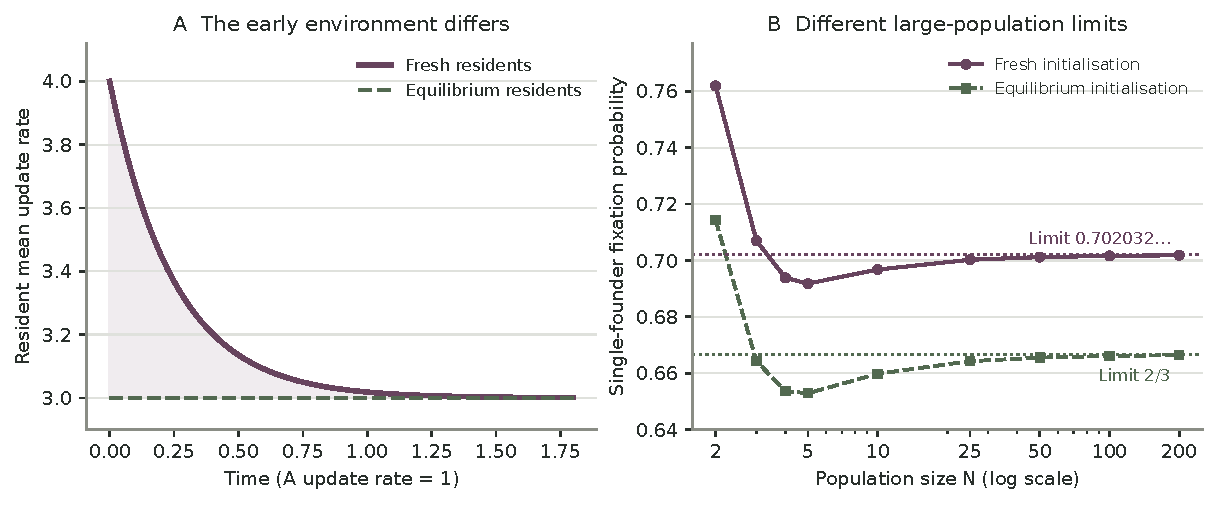
\includegraphics[width=1\linewidth,height=\textheight,keepaspectratio,alt={The constant-rate witness (a=1, resident rates 2 and 6 with equal probabilities). Panel A: under a fresh start the mean resident rate starts at 4 and relaxes to its equilibrium value 3 as 3+e\^{}\{-4t\}. Panel B: what to notice is that fresh-start fixation (upper, purple) approaches 0.70203, not the conjectured 2/3 (lower, green), and that the gap is already visible at N\textbackslash approx10. Points for N\textbackslash le5 are exact rational solutions; larger N are floating sparse solves. Lines between points guide the eye; dotted lines mark the proved limits.}]{../figures/consensus_initialisation.pdf}
\caption{The constant-rate witness (\(a=1\), resident rates \(2\) and
\(6\) with equal probabilities). Panel A: under a fresh start the mean
resident rate starts at \(4\) and relaxes to its equilibrium value \(3\)
as \(3+e^{-4t}\). Panel B: what to notice is that fresh-start fixation
(upper, purple) approaches \(0.70203\), not the conjectured \(2/3\)
(lower, green), and that the gap is already visible at \(N\approx10\).
Points for \(N\le5\) are exact rational solutions; larger \(N\) are
floating sparse solves. Lines between points guide the eye; dotted lines
mark the proved limits.}
\end{figure}

A second witness, \(a=1\) and
\(F=\frac1{10}\delta_2+\frac9{10}\delta_{100}\), has conjectured value
\(941/1000\). Its certified corrected limit lies between
\(0.9874094825209359\) and \(0.9874094825209361\). A short argument also
gives a fully rational proof of strict separation. On \([0,1/10]\),
\(b_F(t)\ge b_F(1/10)>38\), because \(e^{-59/50}>3/10\) by an
alternating Taylor bound. So the limiting lineage dominates a
homogeneous birth--death process with birth rate \(38\) and death rate
\(1\) up to time \(1/10\). After that, Lemma 3.1 applies with
\(\rho=1/2\). Kendall's formula (21) then gives

\[
\liminf_N\alpha_1(N;F)\ge\frac{37}{38+36e^{-37/10}}>\frac{370}{389}>\frac{941}{1000},
\tag{34}
\]

using \(e^{37/10}>40\) from a positive Taylor sum. The verification
script checks every rational inequality in this chain.

\section{5. How large can the error
be?}\label{how-large-can-the-error-be}

Throughout this section the favourable rate \(a\) is constant and the
residents start fresh. Let \(b_0\) be any number with \(a<b_0\le b_-\),
so that every resident rate is at least \(b_0\). Put
\(\gamma=\lambda-a\).

\subsection{5.1. Total excess intensity}\label{total-excess-intensity}

Let \(\chi(t)=b_F(t)-\lambda\) be the excess intensity,
\(D(t)=\int_0^t\chi\) its cumulative value, and \(D=D(\infty)\). The
spectral gap of \(\mathcal L\) is at least \(b_0\). To see this, note
that \(\mu\le(\lambda/b_0)F\), so for every \(f\),
\(\operatorname{Var}_\mu(f)\le\mathbb E_\mu[(f-\mathbb E_Ff)^2]\le(\lambda/b_0)\operatorname{Var}_F(f)\).
Together with (24) this gives
\(\langle f,-\mathcal Lf\rangle_\mu\ge b_0\operatorname{Var}_\mu(f)\).
Hence \(\varrho_\varphi\) is supported in \([b_0,\infty)\), and
\(\chi(t)\le\chi(0)e^{-b_0t}\). Writing \(m_j=\mathbb E_F[R^{-j}]\) and
expanding (9) at \(z=0\) gives \(\widehat h_F(z)=1-m_1z+m_2z^2+O(z^3)\)
and \(\widehat b_F(z)=1/(m_1z)+m_2/m_1^2-1+O(z)\). Therefore

\[
D=\frac{\mathbb E_F[R^{-2}]}{(\mathbb E_F[R^{-1}])^2}-1,
\tag{35}
\]

which is the usual renewal-function constant. Since
\(R^{-2}\le R^{-1}/b_0\),

\[
0\le D\le\frac\lambda{b_0}-1.
\tag{36}
\]

Because \(0\le D(t)\le D\) and \(I_F(t)=\gamma t+D(t)\), equation (4)
yields

\[
\frac\gamma\lambda\le c_F\le\frac\gamma{\gamma+ae^{-D}}\le\frac\gamma{\gamma+ae^{-(\lambda/b_0-1)}}.
\tag{37}
\]

The first inequality is strict for non-degenerate \(F\).

\subsection{5.2. The sharp envelope}\label{the-sharp-envelope}

\textbf{Theorem 3 (sharp envelope at fixed harmonic mean).} Fix
\(0<a<b_0<\lambda\). Over all compactly supported resident-rate laws on
\([b_0,\infty)\) with harmonic mean \(\lambda\), the supremum of \(c_F\)
is

\[
\frac{\lambda-a}{\lambda-a+ae^{-(\lambda/b_0-1)}}.
\tag{38}
\]

The supremum is not attained.

\emph{Proof.} The upper bound is (37). For \(R>\lambda\) let

\[
F_R=p_R\delta_{b_0}+(1-p_R)\delta_R,\qquad
p_R=\frac{b_0(R-\lambda)}{\lambda(R-b_0)}.
\tag{39}
\]

Each \(F_R\) has harmonic mean \(\lambda\). In the notation of (27),
\(\kappa_R=p_RR+(1-p_R)b_0\to\infty\) and
\(C_{p_R}/\kappa_R\to\lambda/b_0-1\) as \(R\to\infty\). Hence
\(I_R(t)\to\gamma t+\lambda/b_0-1\) for every \(t>0\). The integrands in
(4) are bounded by \(e^{-\gamma t}\), so dominated convergence gives the
limit (38). For non-attainment, equality in \(R^{-2}\le R^{-1}/b_0\)
would force \(R=b_0\) almost surely, contradicting \(\lambda>b_0\). So
\(D<\lambda/b_0-1\) for every admissible law, and the last inequality in
(37) is strict. \(\square\)

The extremal family puts almost all of the excess intensity into a
vanishingly short initial boundary layer. Very fast residents redraw
almost at once, and a lineage that is still small at that moment profits
from all of the excess. This, rather than the moment bound (36), is what
makes the envelope sharp for fixation.

\subsection{5.3. The global supremum}\label{the-global-supremum}

Time can be rescaled, so only \(\lambda/a\) matters. Put
\(\xi=\lambda/a-1>0\) and

\[
\Delta(\xi)=\frac{\xi}{\xi+e^{-\xi}}-\frac{\xi}{1+\xi}.
\tag{40}
\]

\textbf{Proposition 5.1 (global supremum).} Over all constant favourable
rates \(a\) and all resident laws whose support is a compact subset of
the open interval \((a,\infty)\) (so
\(\operatorname{supp}F\subset[b_0,\bar b]\) for some
\(a<b_0\le\bar b<\infty\)), the supremum of the single-founder
underestimate \(c_F-(1-a/\lambda)\) equals
\(\Delta(\xi_*)=\max_{\xi>0}\Delta(\xi)\). It is not attained.

\emph{Proof.} \emph{Upper bound.} Let
\(b_0=\min\operatorname{supp}F>a\). If \(\lambda=b_0\), then
\(F=\delta_{b_0}\) and the underestimate is \(0\). Otherwise, Theorem 3
gives strict inequality in (37). The right side of (37) increases with
\(D\), and \(\lambda/b_0-1<\lambda/a-1=\xi\), so
\(c_F<\gamma/(\gamma+ae^{-\xi})\). With \(\gamma=a\xi\) this says
\(c_F-(1-a/\lambda)<\Delta(\xi)\le\Delta(\xi_*)\).

\emph{Approach.} Fix \(\xi>0\), and take \(a=1\) and \(\lambda=1+\xi\).
Choose \(b_n\downarrow1\) with \(b_n<\lambda\). For each \(n\), Theorem
3 provides a finite-rate law with harmonic mean \(\lambda\), minimum
rate \(b_n\), and an underestimate within \(1/n\) of
\(\gamma/(\gamma+e^{-(\lambda/b_n-1)})-\gamma/\lambda\). This quantity
tends to \(\Delta(\xi)\) as \(n\to\infty\). Hence the supremum is at
least \(\Delta(\xi)\) for every \(\xi\), and so at least
\(\Delta(\xi_*)\). \(\square\)

\emph{The maximiser is unique.} Let
\(\Omega(\xi)=(\xi e^{\xi/2}+e^{-\xi/2})/(1+\xi)^{3/2}\). A direct
computation shows that \(\Delta'(\xi)>0\) exactly when
\(\Omega(\xi)<1\). The derivative of \(\Omega\) has the sign of
\(\Phi(\xi)=(\xi^2+2)e^\xi-(\xi+4)\). Since \(\Phi(0)=-2\) and
\(\Phi'(\xi)=(\xi^2+2\xi+2)e^\xi-1>0\), the function \(\Omega\) first
decreases and then increases. As \(\Omega(0)=1\) and
\(\Omega(\xi)\to\infty\), it crosses \(1\) exactly once, at \(\xi_*>0\).
Since \(\Delta\to0\) at both ends, \(\xi_*\) is the unique maximiser.
Rational exponential bounds (Appendix A) certify

\[
\begin{gathered}
1.71891151345837<\xi_*<1.71891151345839,\\
0.2733554343215126<\Delta(\xi_*)<0.2733554343215181.
\end{gathered}
\tag{41}
\]

So the stationary approximation can underestimate single-founder
fixation by amounts arbitrarily close to \(27.3355\) percentage points,
but never by that much. The approach to the supremum is not uniform in
the model. It needs \(b_0\downarrow a\), so the separation ratio
\(\rho=a/b_0\) tends to \(1\). It also needs the fastest resident rate
to grow without bound. Both are physically extreme: real robots signal
for a minimum duration, which caps the resident rate. Section 5.4 treats
such caps. Finally, the result is about limits as \(N\to\infty\); we do
not claim a finite-\(N\) error bound.

\begin{figure}
\centering
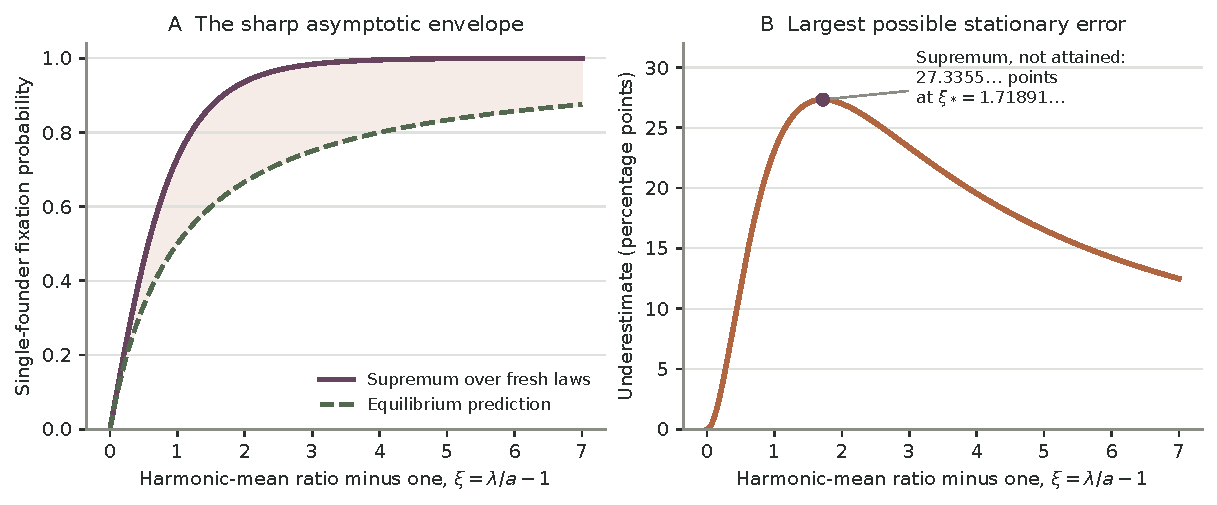
\includegraphics[width=1\linewidth,height=\textheight,keepaspectratio,alt={Panel A: the sharp envelope (38) with b\_0\textbackslash downarrow a (upper, purple), against the stationary prediction \textbackslash xi/(1+\textbackslash xi) (lower, green), as functions of \textbackslash xi=\textbackslash lambda/a-1. The upper curve is a supremum over models, not the fixation curve of any one model. Panel B: their difference, with its maximum of about 27.34 points at \textbackslash xi\_*\textbackslash approx1.719.}]{../figures/consensus_error_envelope.pdf}
\caption{Panel A: the sharp envelope (38) with \(b_0\downarrow a\)
(upper, purple), against the stationary prediction \(\xi/(1+\xi)\)
(lower, green), as functions of \(\xi=\lambda/a-1\). The upper curve is
a supremum over models, not the fixation curve of any one model. Panel
B: their difference, with its maximum of about \(27.34\) points at
\(\xi_*\approx1.719\).}
\end{figure}

\subsection{5.4. The error under a rate
cap}\label{the-error-under-a-rate-cap}

Suppose that every resident rate also satisfies \(R\le\bar b<\infty\).
Then \(X=1/R\) lies in \([1/\bar b,1/b_0]\). Taking expectations in
\((X-1/\bar b)(1/b_0-X)\ge0\) gives the endpoint moment bound

\[
D\le D(b_0,\bar b):=\frac{(\lambda-b_0)(\bar b-\lambda)}{b_0\bar b},
\tag{42}
\]

which is the Bhatia--Davis inequality in the variable \(X\). Hence, by
(37),

\[
c_F-\frac\gamma\lambda\le\frac\gamma{\gamma+ae^{-D(b_0,\bar b)}}-\frac\gamma\lambda.
\tag{43}
\]

Maximising the right side over \(\lambda\in[b_0,\bar b]\) gives a
\emph{proved ceiling} for every law on \([b_0,\bar b]\). The bound (42)
is attained by a law on the two endpoints. The ceiling (43) is not
claimed to be sharp, because the timing of the excess intensity also
matters. Table 3 compares the ceiling with values that are actually
attained: the best law on the two endpoints, optimised over its weight,
and the uniform law.

\begin{longtable}[]{@{}
  >{\raggedleft\arraybackslash}p{(\linewidth - 8\tabcolsep) * \real{0.2000}}
  >{\raggedleft\arraybackslash}p{(\linewidth - 8\tabcolsep) * \real{0.2000}}
  >{\raggedleft\arraybackslash}p{(\linewidth - 8\tabcolsep) * \real{0.2000}}
  >{\raggedleft\arraybackslash}p{(\linewidth - 8\tabcolsep) * \real{0.2000}}
  >{\raggedleft\arraybackslash}p{(\linewidth - 8\tabcolsep) * \real{0.2000}}@{}}
\caption{Single-founder underestimate \(c_F-(1-a/\lambda)\), in
percentage points, under a rate cap. The first two numeric columns are
values attained by specific laws; the last is a proved upper bound over
all laws on \([b_0,\bar b]\). Values are floating-point evaluations of
the exact formulas (29), (4) and (43), computed by
\protect\texttt{stationary\_identity\_and\_caps.py}. The global supremum
\(27.34\) is approached only as \(b_0/a\to1\) and
\(\bar b/b_0\to\infty\).}\tabularnewline
\toprule\noalign{}
\begin{minipage}[b]{\linewidth}\raggedleft
\(b_0/a\)
\end{minipage} & \begin{minipage}[b]{\linewidth}\raggedleft
\(\bar b/b_0\)
\end{minipage} & \begin{minipage}[b]{\linewidth}\raggedleft
Best two-point law (attained)
\end{minipage} & \begin{minipage}[b]{\linewidth}\raggedleft
Uniform law on \([b_0,\bar b]\)
\end{minipage} & \begin{minipage}[b]{\linewidth}\raggedleft
Proved ceiling (43)
\end{minipage} \\
\midrule\noalign{}
\endfirsthead
\toprule\noalign{}
\begin{minipage}[b]{\linewidth}\raggedleft
\(b_0/a\)
\end{minipage} & \begin{minipage}[b]{\linewidth}\raggedleft
\(\bar b/b_0\)
\end{minipage} & \begin{minipage}[b]{\linewidth}\raggedleft
Best two-point law (attained)
\end{minipage} & \begin{minipage}[b]{\linewidth}\raggedleft
Uniform law on \([b_0,\bar b]\)
\end{minipage} & \begin{minipage}[b]{\linewidth}\raggedleft
Proved ceiling (43)
\end{minipage} \\
\midrule\noalign{}
\endhead
\bottomrule\noalign{}
\endlastfoot
1.25 & 2 & 2.08 & 0.68 & 3.12 \\
1.25 & 3 & 4.86 & 1.57 & 7.77 \\
1.25 & 10 & 13.88 & 3.47 & 18.80 \\
1.25 & 100 & 21.37 & 1.72 & 22.22 \\
2 & 2 & 1.66 & 0.54 & 2.74 \\
2 & 3 & 3.59 & 1.13 & 5.95 \\
2 & 10 & 9.40 & 2.24 & 12.51 \\
2 & 100 & 14.03 & 1.07 & 14.54 \\
\end{longtable}

\subsection{5.5. Could simulations have seen the
effect?}\label{could-simulations-have-seen-the-effect}

The source estimates fixation probabilities from \(1000\) simulation
runs per point (Ganesh et al., 2025, Section 4). Near \(p=0.7\), the
standard error of such an estimate is
\(\sqrt{0.7\times0.3/1000}\approx1.45\) percentage points, and a 95\%
interval has half-width about \(2.8\) points. The constant-rate witness
has an asymptotic gap of \(3.54\) points, and at \(N=100\) the computed
gap is \(3.49\) points (Table 5). This is about \(2.4\) standard errors.
A dedicated two-sided test at the 5\% level would detect it with
probability only about two thirds. It would not be evident by eye on a
plotted curve that also carries finite-\(N\) effects. There is a more
basic reason why the source's simulations could not have detected it:
they used the equilibrium start, for which (7) shows that the gap is
zero when the favourable rate is constant. Their Gamma-noise examples
also have overlapping supports, which lie outside our class.

\section{6. Burn-in: pre-ageing the
residents}\label{burn-in-pre-ageing-the-residents}

Suppose that the residents evolve on their own for a time \(\tau\ge0\)
before the \(k\) favourable agents arrive. Their initial law is then
\(\nu_\tau=FP_\tau\), so \(b_{\nu_\tau}(t)=b_F(t+\tau)\). Let \(c_\tau\)
be the single-founder limit. Then
\(I_{\nu_\tau}(t)=\gamma t+\int_\tau^{\tau+t}\chi\). By (26), \(\chi\)
is strictly decreasing when \(F\) is non-degenerate, since
\(\chi'(t)=-\lambda^{-1}\int\xi e^{-\xi t}\varrho_\varphi(d\xi)<0\). So
\(\int_\tau^{\tau+t}\chi\) strictly decreases in \(\tau\) for each
\(t>0\), and by (4) \(c_\tau\) strictly decreases in \(\tau\). Its limit
is the stationary value \(\gamma/\lambda\).

The remaining excess is
\(D_\tau=\int_\tau^\infty\chi\le De^{-b_0\tau}\), because
\(\varrho_\varphi\) is supported in \([b_0,\infty)\). The argument of
(37) gives

\[
\frac\gamma\lambda\le c_\tau\le\frac\gamma{\gamma+a\exp(-D_\tau)}.
\tag{44}
\]

The function \(y\mapsto\gamma/(\gamma+ae^{-y})\) has derivative
\(u/(1+u)^2\) with \(u=(a/\gamma)e^{-y}\). That derivative is at most
\(L\), where \(L=a\gamma/\lambda^2\) if \(\gamma\ge a\) (then \(u\le1\),
where \(u/(1+u)^2\) increases) and \(L=1/4\) otherwise. Hence

\[
0\le c_\tau-\frac\gamma\lambda\le LDe^{-b_0\tau},
\tag{45}
\]

and for an absolute tolerance \(\varepsilon>0\) a sufficient burn-in
time is

\[
\tau\ge\frac1{b_0}\max\Bigl\{0,\ \log\frac{LD}{\varepsilon}\Bigr\}.
\tag{46}
\]

Bounds (45) and (46) concern the single-founder limit \(c_\tau\). For
the \(k\)-founder fixation probability \(p_k(c)=1-(1-c)^k\), write
\(c_0=\gamma/\lambda\), so \(1-c_0=a/\lambda\), and
\(\delta_\tau=c_\tau-c_0\). By the mean value theorem,

\[
0\le p_k(c_\tau)-p_k(c_0)=\Bigl(\frac a\lambda\Bigr)^k-\Bigl(\frac a\lambda-\delta_\tau\Bigr)^k\le k\Bigl(\frac a\lambda\Bigr)^{k-1}LDe^{-b_0\tau},
\]

so a sufficient burn-in for tolerance \(\varepsilon\) in the
\(k\)-founder probability is

\[
\tau\ge\frac1{b_0}\max\Bigl\{0,\ \log\frac{k(a/\lambda)^{k-1}LD}{\varepsilon}\Bigr\}.
\]

This reduces to (46) when \(k=1\).

If \(D=0\), the resident rate is deterministic and no burn-in is needed.
For the witness of Section 4.3, \(D=1/4\), \(b_0=2\) and \(L=2/9\). A
tolerance of \(\varepsilon=10^{-3}\), that is \(0.1\) percentage point,
in the single-founder probability then needs only
\(\tau\ge\frac12\log(55.6)\approx2.01\) mean favourable signalling
times.

This bound has two uses. An experimenter who wants simulations to test
the stationary theory should burn in the residents for this long. A
swarm designer does not need to: in this model, a fresh start only helps
the better option.

\section{7. Random favourable rates}\label{random-favourable-rates}

We now let the favourable rate law \(F_A\) on \([a_-,a_+]\) be
arbitrary, with any initial favourable law \(\nu^A\). Section 7.1
identifies the limit. Section 7.2 treats the equilibrium start that the
source simulated. Section 7.3 shows that fresh residents strictly help.
Section 7.4 reports numerical values.

\subsection{7.1. The limit}\label{the-limit}

Let \(\mathcal Z\) be the branching process of Section 3.4. For
\(s\le T\) and \(x\in[a_-,a_+]\), let \(e^{(T)}_s(x)\) be the
probability that the lineage of a type-\(x\) individual alive at time
\(s\) is extinct by time \(T\). Let
\(\psi^{(T)}(t)=\int e^{(T)}_t(y)F_A(dy)\) be the same probability for a
newborn at time \(t\) with a fresh type. More generally, for
\(z\in[0,1]\) let \(Q^{(T,z)}_s(x)=\mathbb E_{x,s}[z^{Z(T)}]\) and
\(\psi^{(T)}_z(t)=\int Q^{(T,z)}_t(y)F_A(dy)\), so that
\(e^{(T)}=Q^{(T,0)}\).

\textbf{Lemma 7.1 (backward equations).} Write
\(\mathcal E_z(s,v)=\exp\bigl(-\int_s^vb_\nu(t)[1-\psi^{(T)}_z(t)]dt\bigr)\).
Then

\[
Q^{(T,z)}_s(x)=ze^{-x(T-s)}\mathcal E_z(s,T)+\int_s^Txe^{-x(v-s)}\mathcal E_z(s,v)\,dv.
\tag{47}
\]

Consequently, \(s\mapsto Q^{(T,z)}_s(x)\) solves

\[
\frac{d}{ds}Q_s(x)=x[Q_s(x)-1]+b_\nu(s)Q_s(x)\Bigl[1-\int Q_s(y)F_A(dy)\Bigr],
\qquad Q_T(x)=z.
\tag{48}
\]

\emph{Proof.} Types never change, so the remaining lifetime of the
individual is \(\operatorname{Exp}(x)\). Given that lifetime, its
children are born at the points of a Poisson process of intensity
\(b_\nu\), with independent \(F_A\) types. By the branching property, a
child born at time \(t\) contributes an independent factor with mean
\(\psi^{(T)}_z(t)\). The probability generating functional of a Poisson
process gives the factor \(\mathcal E_z\). If the individual is alive at
\(T\) it also contributes a factor \(z\). Summing over death before or
after \(T\) gives (47). Differentiating (47) in \(s\) gives
\(\partial_sQ_s=-x+(x+b_\nu(s)[1-\psi^{(T)}_z(s)])Q_s\), which is (48).
\(\square\)

For a finite favourable law \(F_A=\sum_i\varpi_i\delta_{a_i}\), equation
(48) is the finite system of backward equations that one integrates in
practice. The extinction probabilities
\(e_s(x)=\lim_{T\to\infty}e^{(T)}_s(x)\) exist by monotonicity in \(T\).
By monotone convergence in (47) with \(z=0\),

\[
e_s(x)=\int_s^\infty xe^{-x(v-s)}\exp\Bigl(-\int_s^vb_\nu(t)[1-\psi(t)]dt\Bigr)dv,
\qquad\psi(t)=\int e_t(y)F_A(dy).
\tag{49}
\]

\textbf{Theorem 4 (random favourable rates).} Assume (1). For every
fixed \(k\ge1\),

\[
\lim_{N\to\infty}\alpha_k(N;\nu^A,\nu)=1-\Bigl[\int e_0(x)\,\nu^A(dx)\Bigr]^k.
\tag{50}
\]

\emph{Proof.} Proposition 3.6 identifies the limit as the survival
probability of \(\mathcal Z\). Founder lineages are independent, and
each goes extinct with probability \(\int e_0\,d\nu^A\). \(\square\)

\textbf{Lemma 7.2 (a uniform survival bound).} Let \(\rho=a_+/b_-\).
From any configuration of \(m\) individuals at any time, \(\mathcal Z\)
goes extinct with probability at most \(\rho^m\).

\emph{Proof.} Let \(\Sigma\) be the sum of the types of the living
individuals, so \(\Sigma\le a_+Z\). The generator of \(\mathcal Z\)
applied to \(\rho^Z\) is

\[
b_\nu Z(\rho^{Z+1}-\rho^Z)+\Sigma(\rho^{Z-1}-\rho^Z)=\rho^{Z-1}(1-\rho)(\Sigma-\rho b_\nu Z)\le\rho^{Z-1}(1-\rho)Z(a_+-\rho b_-)=0.
\]

There is no explosion, since births are dominated by a Yule process.
Localising at the exit times from \(\{Z\le K\}\) and letting
\(K\to\infty\) with Fatou's lemma, \(\rho^{Z(t)}\) is a bounded
supermartingale, so \(\mathbb E\rho^{Z(n)}\le\rho^m\). By Lemma 3.5,
\(\rho^{Z(n)}\to\mathbf 1\{\text{extinction}\}\) almost surely, and
bounded convergence gives \(\mathbb P(\text{extinction})\le\rho^m\).
\(\square\)

\subsection{7.2. The equilibrium start}\label{the-equilibrium-start}

\textbf{Lemma 7.3 (equilibrium residents).} If \(\nu=\mu\), then
\(e_s(x)=e(x)\) does not depend on \(s\), and

\[
e(x)=\frac x{x+\lambda c^\ast},
\tag{51}
\]

where \(c^\ast\in(0,1)\) is the unique positive root of
\(\int\lambda(x+\lambda c)^{-1}F_A(dx)=1\). In particular, fresh
favourable founders give the limit \(1-(1-c^\ast)^k=1-\pi^k\), which is
the conjectured value.

\emph{Proof.} With \(b_\mu\equiv\lambda\) the process is
time-homogeneous. So \(e^{(T)}_s\) depends only on \(T-s\), and its
limit \(e_s\) does not depend on \(s\). Then (49) with constant \(\psi\)
gives \(e(x)=x/(x+\lambda c)\) with \(c=1-\psi\). Integrating against
\(F_A\) gives \(c=\int\lambda c/(x+\lambda c)\,F_A(dx)\). By Lemma 7.2,
\(c\ge1-\rho>0\), so after division by \(c\) we get
\(\int\lambda(x+\lambda c)^{-1}F_A(dx)=1\). The left side \(g(c)\) is
continuous and strictly decreasing in \(c\), with
\(g(0+)=\lambda\int x^{-1}F_A(dx)=\lambda m_A>1\) and \(g(1)<1\); so a
root exists in \((0,1)\) and it is unique. Hence \(c=c^\ast\), and (51)
agrees with the source's Theorem 5 in our class. \(\square\)

\textbf{Theorem 6 (equilibrium start: the mean-quality formula).} Assume
(1), and start both opinions from equilibrium: \(\nu=\mu\) and
\(\nu^A=G_A\), as in the source's Section 4.7 simulations. Then for
every fixed \(k\ge1\),

\[
\lim_{N\to\infty}\alpha_k(N;G_A,\mu)=1-\left(\frac{\mathbb E\,T_B}{\mathbb E\,T_A}\right)^k
=1-\left(\frac1{\lambda m_A}\right)^k.
\tag{52}
\]

\emph{Proof.} By Theorem 4 and Lemma 7.3,

\[
\int e\,dG_A=\frac1{m_A}\int\frac1x\cdot\frac x{x+\lambda c^\ast}F_A(dx)
=\frac1{\lambda m_A}\int\frac\lambda{x+\lambda c^\ast}F_A(dx)=\frac1{\lambda m_A},
\]

where the last step is the defining equation of \(c^\ast\). \(\square\)

Theorem 6 says that, from equilibrium, the noisy model has the same
large-population fixation probability as the noise-free model in which
each option's quality equals its mean quality. In the noise-free model,
single-founder fixation tends to \(1-q_B/q_A\), where \(q_A\) and
\(q_B\) are the two qualities. The identity reflects reproductive value.
A type-\(x\) individual has \(\lambda/x\) offspring on average, so the
equilibrium weighting by \(1/x\) is the reproductive-value weighting,
and it makes the type-averaged extinction probability collapse.

\textbf{Corollary 7 (Conjecture 2 under the simulated start).} Under the
hypotheses of Theorem 6, \(1/(\lambda m_A)\le\pi\), with equality if and
only if \(F_A\) is a point mass. Hence, whenever the favourable rates
vary, the equilibrium-start limit strictly exceeds the conjectured
\(1-\pi^k\).

\emph{Proof.} We have \(\pi=\int e\,dF_A\) and
\(1/(\lambda m_A)=\int e\,dG_A=\mathbb E[e(X)X^{-1}]/\mathbb E[X^{-1}]\)
with \(X\sim F_A\). The function \(e\) is strictly increasing and
\(x\mapsto x^{-1}\) is strictly decreasing. Let \(X'\) be an independent
copy of \(X\). Then
\(\operatorname{Cov}(e(X),X^{-1})=\frac12\mathbb E[(e(X)-e(X'))(X^{-1}-X'^{-1})]\).
This is negative unless \(X=X'\) almost surely, that is, unless \(F_A\)
is a point mass. \(\square\)

For the example of Table 1, \(\lambda=3\) and \(m_A=3/2\), so the
equilibrium-start limit is exactly \(1-1/4.5=7/9\). The conjectured
value is \((3+\sqrt{37})/12\). The stationary-identity script certifies
both values in exact rational arithmetic. It also certifies the identity
(52), and the strict inequality of Corollary 7, for three further
favourable and resident laws.

\subsection{7.3. Fresh residents strictly
help}\label{fresh-residents-strictly-help}

\textbf{Corollary 5 (strict fresh-resident advantage).} Assume (1) and
that \(F\) is not a point mass. For every common initial favourable law
\(\nu^A\) and every \(k\ge1\), fresh residents (\(\nu=F\)) give a
strictly larger limit than equilibrium residents (\(\nu=\mu\)). With
\(\nu^A=F_A\) this means that the fresh-start limit strictly exceeds the
conjectured \(1-\pi^k\).

\emph{Proof.} Let \(\chi(t)=b_F(t)-\lambda>0\), by (26). Build both
branching processes on one space. Every individual carries independent
ingredients:

\begin{itemize}
\tightlist
\item
  an \(\operatorname{Exp}(x)\) lifetime;
\item
  a \emph{baseline} Poisson birth stream of rate \(\lambda\);
\item
  an \emph{extra} Poisson birth stream of intensity \(\chi(t)\) in
  absolute time;
\item
  independent \(F_A\) types for the children of each stream.
\end{itemize}

In \(\mathcal Z^F\), an individual's children are the points of both
streams during its life. In \(\mathcal Z^\mu\), they are the baseline
points only, and only individuals descended from the founders through
baseline births belong to \(\mathcal Z^\mu\). Each process has the
correct law: birth rates \(\lambda+\chi=b_F\) and \(\lambda=b_\mu\)
respectively, with independent \(F_A\) types. The genealogy of
\(\mathcal Z^\mu\) is contained in that of \(\mathcal Z^F\), so survival
of \(\mathcal Z^\mu\) implies survival of \(\mathcal Z^F\).

For strictness, fix a founder of type \(x\) and some \(T>0\). Consider
the event that the founder's lifetime lies in \((T,2T)\), its baseline
stream has no point in \((0,2T)\), its extra stream has a point in
\((0,T)\), and the subtree of the first extra child survives. On this
event the founder has no children in \(\mathcal Z^\mu\), whereas its
lineage survives in \(\mathcal Z^F\). The extra child's subtree has
birth rate \(b_F\ge b_-\) and death rates at most \(a_+\). By Lemma 7.2
it survives with probability at least \(1-\rho\), independently of the
founder's own ingredients given the birth time. Write \(e^F_0\) and
\(e^\mu_0\) for the extinction probabilities (49) under the two resident
starts. Hence

\[
e^\mu_0(x)-e^F_0(x)\ge\bigl(e^{-xT}-e^{-2xT}\bigr)e^{-2\lambda T}\Bigl(1-e^{-\int_0^T\chi}\Bigr)(1-\rho)>0.
\]

The restriction applies only to the founder's own streams; all
descendants' streams are unrestricted. Averaging over \(\nu^A\)
preserves strictness, and (50) proves the claim for every \(k\).
\(\square\)

\subsection{7.4. Numerical values and a computable
bracket}\label{numerical-values-and-a-computable-bracket}

For finite favourable laws, (48) can be integrated numerically. Lemma
7.2, conditioned at time \(T\), and the fact that ultimate survival
requires survival at \(T\) give the bracket

\[
1-\Bigl[\int Q^{(T,\rho)}_0\,d\nu^A\Bigr]^k
\le\lim_{N\to\infty}\alpha_k
\le1-\Bigl[\int Q^{(T,0)}_0\,d\nu^A\Bigr]^k.
\tag{53}
\]

By Lemma 3.5, both sides converge to the limit as integer
\(T\to\infty\). The inequalities (53) are proved. The \emph{values} we
report from them are numerical, not certified: we integrate (48) with an
ordinary floating-point solver (SciPy's DOP853, cross-checked with
Radau), which supplies no rigorous error bound. For the example of Table
1, with fresh residents and fresh favourable founders, the numerical
endpoints of (53) are \(0.7841882234\) and \(0.7842430477\) at \(T=4\),
and \(0.7842272885\) and \(0.7842272947\) at \(T=8\).

Exact finite-population calculations support Theorems 4 and 6. Table 4
reports the probability that a single favourable founder fixes in the
count chain with two favourable and two resident rates. For \(N\le5\)
the values are exact rational solutions; for larger \(N\) they are
floating sparse solves with recorded residuals below \(10^{-9}\).

\begin{longtable}[]{@{}
  >{\raggedleft\arraybackslash}p{(\linewidth - 8\tabcolsep) * \real{0.2000}}
  >{\raggedleft\arraybackslash}p{(\linewidth - 8\tabcolsep) * \real{0.2000}}
  >{\raggedleft\arraybackslash}p{(\linewidth - 8\tabcolsep) * \real{0.2000}}
  >{\raggedleft\arraybackslash}p{(\linewidth - 8\tabcolsep) * \real{0.2000}}
  >{\raggedleft\arraybackslash}p{(\linewidth - 8\tabcolsep) * \real{0.2000}}@{}}
\caption{Single-founder fixation in the finite population for the
example of Table 1, under the four starts. The last row gives the
limits: exact closed forms where available, otherwise the numerical
value of (53) at \(T=12\).}\tabularnewline
\toprule\noalign{}
\begin{minipage}[b]{\linewidth}\raggedleft
\(N\)
\end{minipage} & \begin{minipage}[b]{\linewidth}\raggedleft
fresh / fresh
\end{minipage} & \begin{minipage}[b]{\linewidth}\raggedleft
fresh founders, equilibrium residents
\end{minipage} & \begin{minipage}[b]{\linewidth}\raggedleft
equilibrium / equilibrium
\end{minipage} & \begin{minipage}[b]{\linewidth}\raggedleft
equilibrium founders, fresh residents
\end{minipage} \\
\midrule\noalign{}
\endfirsthead
\toprule\noalign{}
\begin{minipage}[b]{\linewidth}\raggedleft
\(N\)
\end{minipage} & \begin{minipage}[b]{\linewidth}\raggedleft
fresh / fresh
\end{minipage} & \begin{minipage}[b]{\linewidth}\raggedleft
fresh founders, equilibrium residents
\end{minipage} & \begin{minipage}[b]{\linewidth}\raggedleft
equilibrium / equilibrium
\end{minipage} & \begin{minipage}[b]{\linewidth}\raggedleft
equilibrium founders, fresh residents
\end{minipage} \\
\midrule\noalign{}
\endhead
\bottomrule\noalign{}
\endlastfoot
2 & \(1108/1365\) & \(703/910\) & \(1081/1365\) & \(3392/4095\) \\
3 & 0.7804688061 & 0.7465156976 & 0.7673674466 & 0.7989468709 \\
4 & 0.7766495256 & 0.7449666725 & 0.7660039698 & 0.7954392892 \\
5 & 0.7774833222 & 0.7469228746 & 0.7679767124 & 0.7963395208 \\
10 & 0.7813643381 & 0.7526212169 & 0.7736076748 & 0.8002278429 \\
25 & 0.7832269088 & 0.7553742164 & 0.7762973435 & 0.8020667952 \\
50 & 0.7837472904 & 0.7561624295 & 0.7770642809 & 0.8025784494 \\
100 & 0.7839920281 & 0.7565360172 & 0.7774273437 & 0.8028187952 \\
\(\infty\) & 0.7842272930 & \((3+\sqrt{37})/12=0.7568968775\) &
\(7/9=0.7777777778\) & 0.8030496711 \\
\end{longtable}

\section{8. Deterministic verification of the constant-rate
witness}\label{deterministic-verification-of-the-constant-rate-witness}

For two resident rates and a constant favourable rate, the finite
population reduces exactly to states \((m,j)\). Here \(m\) is the number
of favourable vertices and \(j\) the number of slow residents among the
other \(n=N-m\). Write \(r_1<r_2\) for the slow and fast rates and \(p\)
for the probability of drawing the slow rate. The state-changing rates
are:

{\def\LTcaptype{none} % do not increment counter
\begin{longtable}[]{@{}lr@{}}
\toprule\noalign{}
New state & Rate \\
\midrule\noalign{}
\endhead
\bottomrule\noalign{}
\endlastfoot
\((m-1,j+1)\) & \(amnp/(N-1)\) \\
\((m-1,j)\) & \(amn(1-p)/(N-1)\) \\
\((m+1,j-1)\) & \(r_1jm/(N-1)\) \\
\((m+1,j)\) & \(r_2(n-j)m/(N-1)\) \\
\((m,j-1)\) & \(r_1j(n-1)(1-p)/(N-1)\) \\
\((m,j+1)\) & \(r_2(n-j)(n-1)p/(N-1)\) \\
\end{longtable}
}

The verification script solves the resulting harmonic equations exactly
in rational arithmetic for \(N=2,3,4,5\). Every equation has zero exact
residual. A separate implementation enumerates labelled vertex
configurations for \(N=2,3,4\), and its floating results agree with the
exact values. Larger populations are solved by deterministic sparse
linear algebra, with residuals recorded.

For \(a=1\) and \(F=(\delta_2+\delta_6)/2\), the exact fresh-start
probabilities are \(16/21\), \(2864/4051\), \(443968/639901\) and
\(310846319872/449354284245\) for \(N=2,3,4,5\). Their initial decrease
shows that convergence need not be monotone in \(N\). Larger values,
rounded to ten decimals, are:

\begin{longtable}[]{@{}
  >{\raggedleft\arraybackslash}p{(\linewidth - 8\tabcolsep) * \real{0.2000}}
  >{\raggedleft\arraybackslash}p{(\linewidth - 8\tabcolsep) * \real{0.2000}}
  >{\raggedleft\arraybackslash}p{(\linewidth - 8\tabcolsep) * \real{0.2000}}
  >{\raggedleft\arraybackslash}p{(\linewidth - 8\tabcolsep) * \real{0.2000}}
  >{\raggedleft\arraybackslash}p{(\linewidth - 8\tabcolsep) * \real{0.2000}}@{}}
\caption{Constant-rate witness: finite-\(N\) fixation probabilities.
Floating values are rounded to ten decimals; the eleventh and twelfth
decimals can vary by one unit across NumPy/SciPy
versions.}\tabularnewline
\toprule\noalign{}
\begin{minipage}[b]{\linewidth}\raggedleft
\(N\)
\end{minipage} & \begin{minipage}[b]{\linewidth}\raggedleft
Fresh residents
\end{minipage} & \begin{minipage}[b]{\linewidth}\raggedleft
Gap to limit
\end{minipage} & \begin{minipage}[b]{\linewidth}\raggedleft
Equilibrium residents
\end{minipage} & \begin{minipage}[b]{\linewidth}\raggedleft
Gap to \(2/3\)
\end{minipage} \\
\midrule\noalign{}
\endfirsthead
\toprule\noalign{}
\begin{minipage}[b]{\linewidth}\raggedleft
\(N\)
\end{minipage} & \begin{minipage}[b]{\linewidth}\raggedleft
Fresh residents
\end{minipage} & \begin{minipage}[b]{\linewidth}\raggedleft
Gap to limit
\end{minipage} & \begin{minipage}[b]{\linewidth}\raggedleft
Equilibrium residents
\end{minipage} & \begin{minipage}[b]{\linewidth}\raggedleft
Gap to \(2/3\)
\end{minipage} \\
\midrule\noalign{}
\endhead
\bottomrule\noalign{}
\endlastfoot
10 & 0.6967465143 & \(5.29\times10^{-3}\) & 0.6597969966 &
\(6.87\times10^{-3}\) \\
25 & 0.7002259952 & \(1.81\times10^{-3}\) & 0.6642598910 &
\(2.41\times10^{-3}\) \\
50 & 0.7011711989 & \(8.61\times10^{-4}\) & 0.6655113963 &
\(1.16\times10^{-3}\) \\
100 & 0.7016113989 & \(4.21\times10^{-4}\) & 0.6661003029 &
\(5.66\times10^{-4}\) \\
200 & 0.7018240813 & \(2.08\times10^{-4}\) & 0.6663862149 &
\(2.80\times10^{-4}\) \\
\(\infty\) & 0.7020320539 & & \(2/3\) & \\
\end{longtable}

Doubling \(N\) from \(100\) to \(200\) roughly halves both gaps, which
is consistent with an \(O(1/N)\) rate. We do not prove such a rate. The
finite-\(N\) values support the construction, but they do not prove the
limit theorem. The decimal intervals for the limits and for the global
maximiser are separately certified by exact rational arithmetic
(Appendix A).

A basic normalisation check is the deterministic resident law
\(F=\delta_b\). The fresh and equilibrium laws then coincide,
\(b_F(t)=b\), equation (4) gives \(c=1-a/b\), and Theorem 1 reduces to
the usual biased-voter fixation limit. Multiplying all rates by a
positive constant only rescales time and leaves every fixation formula
unchanged.

\section{9. Discussion}\label{discussion}

\textbf{What is resolved.} Within the class (1) on complete graphs,
Conjecture 2 holds exactly when residents start in equilibrium and
favourable founders start fresh. That hybrid start is used by neither
the conjecture nor the source's simulations. Under the stated fresh
start the conjecture is false, whenever resident rates vary, by
Corollary 5 and Theorem 2. Under the simulated equilibrium start it is
true for a constant favourable rate, by (7). It is false for varied
favourable rates, by Corollary 7, where the correct limit is the
mean-quality formula of Theorem 6. Under both the fresh and the
equilibrium start, the conjectured value is an underestimate. The
source's Theorem 5, a calculation of extinction in its stated branching
process, is untouched. What fails is the identification of fresh finite
populations with that stationary process.

\textbf{Fair reading of the source.} One can argue that the conjecture
was \emph{meant} to describe the equilibrium regime and that ``sampled
as above'' is a drafting slip. Section 4.7 of the source supports that
reading. Even then our results matter in two ways. First, for varied
favourable rates the conjectured formula is not the equilibrium answer
either (Corollary 7). Second, the fresh start is the natural start for a
swarm that begins a decision, and the paper quantifies how much it
helps.

\textbf{The general lesson.} Equilibrium approximations are routinely
applied to systems that start fresh. When individuals hold their states
for random times, the equilibrium snapshot is length-biased. A quantity
decided in the early transient, such as the survival of a rare lineage,
then differs at leading order from its stationary prediction. Burn-in
removes the difference, at an exponential rate set by the spectral gap
(Section 6).

\textbf{Open problems.}

\begin{enumerate}
\def\labelenumi{\arabic{enumi}.}
\tightlist
\item
  \emph{Overlapping supports.} If some favourable rates exceed some
  resident rates, the uniform comparison of Lemma 3.1 fails, and we have
  no substitute bridge from early survival to fixation. This is the
  generic case for noisy measurements of nearby qualities, including the
  source's Gamma-noise examples. We expect the transient mechanism to
  persist there, but we have not proved it.
\item
  \emph{Non-complete graphs.} On sparse, regular or geometric graphs,
  the early-transient mechanism should persist locally, but the limit
  formula will not carry over directly. The source also leaves general
  graphs open.
\item
  \emph{A sharp envelope under a rate cap.} Table 3 brackets the worst
  case between attained values and the ceiling (43). The exact extremum
  over laws on \([b_0,\bar b]\) is an optimal-timing problem that we
  have not solved.
\item
  \emph{A finite-\(N\) rate.} Tables 4 and 5 suggest an \(O(1/N)\)
  approach to the limit. An explicit bound would make the corrections
  usable for swarms of tens to hundreds of agents.
\item
  \emph{Non-exponential signalling.} For signalling laws with increasing
  failure rate, the fresh-start renewal intensity can lie below its
  equilibrium value at first. The direction of the bias could then
  reverse.
\end{enumerate}

\section{Declarations}\label{declarations}

\textbf{Author.} Anonymous.

\textbf{Version and status.} Version 1.0.0-candidate, an unrefereed
research candidate. DOI: \url{https://doi.org/10.5281/zenodo.23687032}.

\textbf{AI provenance.} This manuscript was produced with AI systems
based on large language models. They drafted the text and proofs, wrote
the verification scripts, and carried out the literature and citation
checks. The revision responds to five internal AI review reports and one
review by a model from a different family. The proofs have not been
formalised in a proof assistant or refereed by human experts. No human
author takes responsibility for the mathematics; readers should treat
the results as a research draft to be checked. Every reference was
verified against its Crossref record.

\textbf{Data and code availability.} Four Python scripts, using the
standard library or NumPy/SciPy, reproduce every number in this paper.
They are archived with this manuscript at
\url{https://doi.org/10.5281/zenodo.23687032} (version 1.0.0-candidate)
and in the repository
\url{https://github.com/ipitchford/initialisation-dependent-fixation}
(tag \texttt{v1.0.0-candidate}), whose README lists the commands.
\texttt{consensus/certify\_limits.py} gives the rational certificates of
Appendix A. \texttt{consensus/evidence/verify\_finite\_n.py} solves the
scalar finite-population chains and checks the rational chain (34).
\texttt{consensus/evidence/multitype\_bracket.py} integrates (48) for
the bracket (53).
\texttt{consensus/evidence/stationary\_identity\_and\_caps.py} gives the
exact certification of Theorem 6 and Corollary 7, the multitype
finite-population chain of Table 4, and the rate-cap values of Table 3.
No stochastic simulation is used.

\textbf{Competing interests and funding.} None.

\section{Appendix A. Rational
certificates}\label{appendix-a.-rational-certificates}

All certified decimals in this paper come from exact rational enclosures
computed with Python's \texttt{fractions} module. For \(x\ge0\) the
script encloses \(e^x\) between a Taylor polynomial of degree \(n\) and
that polynomial plus a geometric tail bound,
\(x^{n+1}/((n+1)!\,(1-x/(n+2)))\), valid for \(x<n+2\). The series (29)
has positive terms with increasing denominators \(\omega+j\). Its tail
after \(100\) terms is therefore bounded by the next term divided by
\(1-\zeta/102\).

These enclosures give rational bounds on \(c_F^{-1}\), and hence on
\(c_F\). For the global supremum, the script brackets \(\xi_*\) by
checking the sign of \(e^{-\xi}(1+\xi)^3-(\xi+e^{-\xi})^2\), which has
the sign of \(\Delta'\), at the two rational endpoints in (41). It
bounds \(\Delta(\xi_*)\) using the monotonicity of
\(\xi/(\xi+e^{-\xi})\) and \(\xi/(1+\xi)\). The complete fractions, with
numerators and denominators of several hundred digits, are stored in
\texttt{certified\_limits.json}. The certified decimal brackets are:

\begin{itemize}
\tightlist
\item
  constant-rate witness: the lower and upper rational bounds on \(c_F\)
  agree to 30 significant digits,
  \(c_F=0.702032053928212711530878678865\ldots\);
\item
  second witness: likewise,
  \(c_F=0.987409482520935991411990627158\ldots\);
\item
  maximiser: \(\xi_*\in(1.71891151345837,\ 1.71891151345839)\);
\item
  supremum:
  \(\Delta(\xi_*)\in(0.273355434321512683887747,\ 0.273355434321518094791934)\).
\end{itemize}

For Theorem 6, the script brackets \(c^\ast\) to width \(10^{-40}\) by
rational bisection, using the strictly decreasing function
\(c\mapsto\int\lambda(x+\lambda c)^{-1}F_A(dx)\). Both fixation formulas
are increasing in \(c\), so the bracket gives certified enclosures.
These contain \(7/9\) and \((3+\sqrt{37})/12\) for the example of Table
1.

\section{References}\label{references}

Alexandre, A., Abbara, A., Fruet, C., Loverdo, C., \& Bitbol, A.-F.
(2025). Bridging Wright--Fisher and Moran models. \emph{Journal of
Theoretical Biology, 599}, 112030.
\url{https://doi.org/10.1016/j.jtbi.2024.112030}

Athreya, K. B., \& Ney, P. E. (1972). \emph{Branching processes}.
Springer. \url{https://doi.org/10.1007/978-3-642-65371-1}

Brown, M. (1980). Bounds, inequalities, and monotonicity properties for
some specialized renewal processes. \emph{The Annals of Probability,
8}(2), 227--240. \url{https://doi.org/10.1214/aop/1176994773}

Ethier, S. N., \& Kurtz, T. G. (1986). \emph{Markov processes:
Characterization and convergence}. Wiley.
\url{https://doi.org/10.1002/9780470316658}

Fernández-Gracia, J., Eguíluz, V. M., \& San Miguel, M. (2011). Update
rules and interevent time distributions: Slow ordering versus no
ordering in the voter model. \emph{Physical Review E, 84}(1), 015103.
\url{https://doi.org/10.1103/PhysRevE.84.015103}

Ganesh, A., Hauert, S., \& Valla, E. (2025). Consensus in the weighted
voter model with noise-free and noisy observations. \emph{Swarm
Intelligence, 19}(3), 173--214.
\url{https://doi.org/10.1007/s11721-025-00248-z}

Hubbarde, J. E., Wild, G., \& Wahl, L. M. (2007). Fixation probabilities
when generation times are variable: The burst--death model.
\emph{Genetics, 176}(3), 1703--1712.
\url{https://doi.org/10.1534/genetics.107.072009}

Jafarpour, F., Levien, E., \& Amir, A. (2023). Evolutionary dynamics in
non-Markovian models of microbial populations. \emph{Physical Review E,
108}(3), 034402. \url{https://doi.org/10.1103/PhysRevE.108.034402}

Karsai, M., Kivelä, M., Pan, R. K., Kaski, K., Kertész, J., Barabási,
A.-L., \& Saramäki, J. (2011). Small but slow world: How network
topology and burstiness slow down spreading. \emph{Physical Review E,
83}(2), 025102. \url{https://doi.org/10.1103/PhysRevE.83.025102}

Kendall, D. G. (1948). On the generalized ``birth-and-death'' process.
\emph{The Annals of Mathematical Statistics, 19}(1), 1--15.
\url{https://doi.org/10.1214/aoms/1177730285}

Pal, A., Kostinski, S., \& Reuveni, S. (2022). The inspection paradox in
stochastic resetting. \emph{Journal of Physics A: Mathematical and
Theoretical, 55}(2), 021001.
\url{https://doi.org/10.1088/1751-8121/ac3cdf}

Shpak, M. (2007). Selection against demographic stochasticity in
age-structured populations. \emph{Genetics, 177}(4), 2181--2194.
\url{https://doi.org/10.1534/genetics.107.080747}

Stark, H.-U., Tessone, C. J., \& Schweitzer, F. (2008). Decelerating
microdynamics can accelerate macrodynamics in the voter model.
\emph{Physical Review Letters, 101}(1), 018701.
\url{https://doi.org/10.1103/PhysRevLett.101.018701}

Uecker, H., \& Hermisson, J. (2011). On the fixation process of a
beneficial mutation in a variable environment. \emph{Genetics, 188}(4),
915--930. \url{https://doi.org/10.1534/genetics.110.124297}

Valentini, G., Ferrante, E., \& Dorigo, M. (2017). The best-of-n problem
in robot swarms: Formalization, state of the art, and novel
perspectives. \emph{Frontiers in Robotics and AI}, 4, article 9.
\url{https://doi.org/10.3389/frobt.2017.00009}

White, K. P. (1997). An effective truncation heuristic for bias
reduction in simulation output. \emph{Simulation, 69}(6), 323--334.
\url{https://doi.org/10.1177/003754979706900601}

\end{document}
